% manuscript.tex
% Taylor & Francis Interact layout + APA author-year (apacite)
% IJGS Software Tool Article (v3). Do not edit paper-taf-v2/ or paper-taylor-and-francis/.

\documentclass{interact}

\usepackage[T1]{fontenc}
\usepackage[utf8]{inputenc}
\usepackage{epstopdf} 
\usepackage{graphicx}
\usepackage{booktabs}
\usepackage{array}
\usepackage{tabularx}
\usepackage{amsmath}
\usepackage{amssymb}
\usepackage{url}
\usepackage{xcolor}
\usepackage{mdframed}
\usepackage{setspace}

% Slightly more open line spacing for readability
\setstretch{1.25}

% Light gray callout for NLG quotes: box matches default quote width
\definecolor{quoteboxbg}{gray}{0.94}
\mdfdefinestyle{quotebox}{%
  backgroundcolor=quoteboxbg,
  hidealllines=true,
  leftmargin=\leftmargin,
  rightmargin=\leftmargin,
  innertopmargin=10pt,
  innerbottommargin=10pt,
  innerleftmargin=10pt,
  innerrightmargin=10pt,
  skipabove=\topsep,
  skipbelow=\topsep,
}
\renewenvironment{quote}{%
  \begin{mdframed}[style=quotebox]%
}{%
  \end{mdframed}%
}

% Float placement: prefer top of page, keep floats near their callouts,
% and flush deferred floats before major section breaks when needed.
\usepackage{flafter}
\usepackage{placeins}
\renewcommand{\topfraction}{0.95}
\renewcommand{\bottomfraction}{0.8}
\renewcommand{\textfraction}{0.05}
\renewcommand{\floatpagefraction}{0.8}
\setcounter{topnumber}{3}
\setcounter{bottomnumber}{2}
\setcounter{totalnumber}{4}
\setlength{\floatsep}{4pt plus 1pt minus 1pt}
\setlength{\textfloatsep}{8pt plus 2pt minus 2pt}
\setlength{\intextsep}{8pt plus 2pt minus 2pt}
\raggedbottom

% APA author-year (Taylor & Francis Interact + APA)
\usepackage[natbibapa,nodoi]{apacite}
\setlength\bibhang{12pt}
\renewcommand\bibliographytypesize{\fontsize{10}{12}\selectfont}

\usepackage{hyperref}

\begin{document}

\articletype{Software Tool Article}

\title{CADEMAS-ML: A Software Tool for Context-Aware Cooperative and Explainable Automated Decision-Making}

\author{
\name{Pavel Novoa-Hern\'{a}ndez\textsuperscript{a}\thanks{CONTACT Pavel Novoa-Hern\'{a}ndez. Email: pnovoahe@ull.edu.es} and David A. Pelta\textsuperscript{b}}
\affil{\textsuperscript{a}Dept. Computer Engineering and Systems, Universidad de La Laguna, San Crist\'{o}bal de La Laguna, Spain; \textsuperscript{b}Dept. Computer Science and Artificial Intelligence, Universidad de Granada, Granada, Spain}
}

\maketitle

\begin{abstract}
  Complex real-world decision problems often involve multiple decision-making actors that must combine their assessments while accounting for the organizational, operational, and strategic context surrounding the problem. The Cooperative Automated Decision-Making Systems (CADEMAS) framework was recently proposed to represent this form of cooperative and context-aware decision-making. However, previous CADEMAS instantiations cover only specific configurations of a framework that allows substantially broader combinations of automated decision components, contextual models, and aggregation mechanisms. This flexibility, while valuable for practical applications, also makes the framework difficult to operationalize without dedicated software support. This paper presents CADEMAS-ML, a software tool that implements a configurable class of CADEMAS systems in which automated decision-making components are machine learning models and contextual knowledge is represented through fuzzy logic. The tool supports the integration and weighting of multiple predictive models, configurable fuzzy context models, alternative aggregation operators, and an adjustable trade-off between predictive risk and contextual suitability. CADEMAS-ML also incorporates explainability and robustness analysis to support the inspection and assessment of resulting decisions. An employee attrition case study illustrates how the same predictive evidence can lead to different prioritizations under alternative contextual scenarios.
\end{abstract}

\begin{keywords}
automated decision-making systems; fuzzy decision making; context-aware decision support; machine learning; prioritization; cooperative systems
\end{keywords}

\section{Introduction}\label{sec:intro}

Decision-making in real-world organizations is rarely a matter of applying a single analytical model to a well-defined set of inputs. Complex decisions often involve multiple actors, organizational units, or analytical components that contribute different pieces of evidence to the same problem. These contributions may reflect different objectives, information sources, areas of expertise, or levels of reliability, and therefore need to be coordinated before they can support a coherent course of action. This has long motivated the development of cooperative and multi-agent decision-support systems, in which heterogeneous decision components can contribute to a common decision process \citep{Vahidov2004,bui1999agent}. More recent discussions of automated decision-making (ADM) likewise emphasize that algorithmic outputs are embedded in organizational processes rather than existing independently of them \citep{EIP2022,Tariq2024a}.

This organizational perspective becomes particularly important when automated decision-making is used to support prediction, classification, or risk assessment. An automated decision-making component can produce a probability, rating, recommendation, or risk score, but such an output does not by itself determine how the result should be acted upon. The appropriate course of action may depend on factors that are external to the predictive model, including organizational priorities, available resources, departmental objectives, regulatory constraints, or the strategic conditions under which the decision is made. Consequently, the same predictive assessment may have different implications under different circumstances. This distinction between the evidence provided by an automated model and the conditions under which that evidence is interpreted is particularly relevant in organizational decision-support settings, where decisions are embedded in broader operational and institutional contexts \citep{Tariq2024a,Deliu2026}.

Cooperation among automated decision components can therefore be understood as more than the aggregation of several predictions. Different components may provide complementary views of the cases under consideration, while the final decision may also need to reflect contextual knowledge provided by domain experts or organizational policies. In multiperson and group decision-support research, heterogeneous sources of information and preferences have traditionally been combined through aggregation, negotiation, and consensus-seeking mechanisms \citep{Salo1995,HerreraViedma2002}. Similar principles can be extended to automated settings, where the cooperating components may be software-based decision units rather than human decision makers. Agent-based decision-support architectures have, for example, explored the coordination of heterogeneous and distributed decision-support components within organizational workflows \citep{Sycara1998,Vahidov2004}.

Contextual knowledge introduces an additional challenge because it is not always naturally expressed through precise numerical relationships \citep{boos2024conceptualizing}. Experts and decision makers frequently reason in terms such as ``high priority,'' ``moderate relevance,'' ``limited resources,'' or ``strong strategic alignment.'' Fuzzy logic provides a well-established formal basis for representing such concepts through linguistic variables and gradual membership functions \citep{zadeh1975concept}. This capability has made fuzzy approaches particularly useful in decision-support systems where quantitative information must be combined with expert knowledge and imprecise or linguistic assessments \citep{Lamata2020,PerezCanedo2023}. Rather than imposing rigid thresholds, fuzzy representations allow contextual conditions to influence a decision to different degrees, which is well suited to scenarios in which organizational priorities vary with the circumstances.

These considerations motivated the development of the Cooperative Automated Decision-Making Systems (CADEMAS) framework proposed by \citet{NovoaHernandez2026}. CADEMAS provides a conceptual framework for coordinating heterogeneous automated decision-making components while explicitly incorporating the context in which their outputs are interpreted. Its central principle is to distinguish between the generation and integration of decision evidence and the contextual evaluation of that evidence. Multiple automated decision units can therefore contribute to a collective assessment, while a separate contextual layer represents organizational priorities, policies, or scenario-dependent considerations. The resulting decision is obtained by combining these two sources of information rather than treating the predictive assessment as an isolated or definitive outcome.

The original CADEMAS formulation was illustrated through a corporate insolvency prediction problem, demonstrating how several automated decision units could contribute to a common assessment while contextual information influenced the resulting prioritization. More recently, \citet{Godz2026} instantiated the framework in an employee-attrition prevention scenario, using machine-learning models developed from different organizational perspectives as the automated decision units and incorporating organizational scenarios through a fuzzy context layer. These studies provide evidence that the framework can be applied to practical decision problems in which predictive information and contextual considerations need to be combined. At the same time, they represent specific instantiations of a framework whose design permits substantially broader combinations of decision units, weighting schemes, contextual models, aggregation operators, and decision policies.

This flexibility is both a strength of CADEMAS and a practical challenge. A new application requires decisions about how the automated components should be defined, how their outputs should be aligned and integrated, how contextual conditions should be represented, and how the different sources of information should ultimately influence the prioritization of cases. These choices are conceptually part of the framework, but their implementation must otherwise be developed separately for each application. As the number of configurable elements increases, reproducing and experimenting with alternative CADEMAS configurations can become increasingly demanding for researchers, practitioners, and decision makers. A dedicated software implementation can therefore serve not only as a means of reducing implementation effort, but also as a common environment in which different configurations of the framework can be constructed, inspected, compared, and reproduced.

The need for such an environment is particularly relevant for machine-learning-based instantiations of CADEMAS. Machine-learning models provide effective mechanisms for extracting predictive evidence from historical data, but their outputs introduce additional requirements when they become part of a decision-support process. In particular, users may need to understand why a particular case receives a given prediction and how changes in the underlying information affect the result. Explainable artificial intelligence has consequently become an important area of research for the practical use of machine-learning models, particularly when predictions contribute to decisions with organizational or human consequences \citep{Arrieta2020}. Model-agnostic approaches such as SHAP provide local feature attributions that can help users inspect the factors contributing to individual predictions \citep{Lundberg2017,Lundberg2020}. In a cooperative decision system, however, such explanations are only one part of the analysis: users may also need to understand how the predictive outputs interact with contextual assumptions and whether the resulting prioritization remains stable when those assumptions change.

Robustness analysis is therefore another relevant capability for context-aware decision support. In CADEMAS, the final prioritization depends not only on predictive evidence but also on contextual definitions, aggregation mechanisms, and the relative importance assigned to predictive and contextual information. Changes in these elements may alter the ordering of cases even when the underlying predictive models remain unchanged. Allowing users to examine such changes can provide information about the stability of the resulting decisions and expose cases whose prioritization is particularly sensitive to the adopted policy configuration \citep{Arrieta2020}.

Motivated by these considerations, and with the aim of addressing the practical needs described above, this paper presents CADEMAS-ML, a software tool designed to operationalize a configurable class of CADEMAS systems in which automated decision-making components are implemented as machine-learning models and contextual knowledge is represented through fuzzy logic.
The tool integrates multiple predictive models into a collective risk assessment, provides configurable mechanisms for representing and aggregating contextual conditions, and combines predictive risk with contextual suitability through an explicit trade-off mechanism. In addition to these core CADEMAS capabilities, this work proposes explainability and robustness analysis as natural extensions of the framework, given their relevance to the practical inspection and assessment of context-aware decisions. Both capabilities are incorporated into CADEMAS-ML as complementary components of the decision-support workflow. The objective is to provide a reusable software environment through which cooperative and context-aware decision-making configurations can be implemented and analyzed.

The main contributions of this work are as follows:

\begin{itemize}
    \item \textit{A software implementation of CADEMAS.} CADEMAS-ML provides a reusable and configurable implementation of a class of CADEMAS systems in which machine-learning models act as automated decision-making components and fuzzy logic is used to represent contextual knowledge.
    
    \item \textit{Configurable cooperative and context-aware decision support.} The tool allows for integrating heterogeneous predictive models, performance-based model weighting, fuzzy contextual representations, alternative aggregation mechanisms, and an explicit trade-off between predictive risk and contextual suitability.
    
    \item \textit{Explainability and robustness analysis.} The tool extends the decision-support workflow with case-level explanations and mechanisms for analyzing how prioritization outcomes change under alternative contextual and policy configurations.
    
    \item \textit{A reproducible software demonstration.} The capabilities of the tool are demonstrated in an employee-attrition scenario involving multiple organizational predictive models and alternative contextual configurations, illustrating how identical predictive evidence can lead to different prioritization outcomes when the decision context changes.
\end{itemize}

The resulting tool provides a bridge between the conceptual principles of CADEMAS and their practical use in machine-learning-based decision-support applications. Rather than restricting the framework to a single predefined configuration, CADEMAS-ML makes several of its principal design choices explicit and configurable. This allows users (e.g., practitioners and decision-makers) to construct alternative decision policies while preserving the separation between predictive evidence and contextual evaluation that characterizes CADEMAS. The inclusion of explainability and robustness analysis further supports a decision-support workflow in which a prioritization is not only generated, but can also be inspected, justified, and examined under alternative assumptions.

The remainder of the paper is organized as follows. Section~\ref{sec:background} reviews the CADEMAS framework and related work on cooperative and fuzzy decision-support systems. Section~\ref{sec:methods} describes how CADEMAS-ML instantiates that framework for case prioritization and presents the resulting software architecture. Section~\ref{sec:results} introduces an employee-attrition case study and then shows the main functionalities of the tool through that example. Finally, Section~\ref{sec:discussion} summarizes the main findings and discusses implications and future directions.

\section{Background and related works}\label{sec:background}

This section sets out the conceptual foundations on which CADEMAS-ML builds. We first revisit the CADEMAS framework in its general form (Section~\ref{sec:cademas}). We then situate the tool among related cooperative-decision frameworks and application-oriented decision-support systems, clarifying the gap it is designed to fill (Section~\ref{sec:related}).

\subsection{CADEMAS framework}\label{sec:cademas}

As introduced in Section~\ref{sec:intro}, CADEMAS \citep{NovoaHernandez2026} provides a general conceptual and architectural framework for structuring cooperation among heterogeneous Automated Decision-Making (ADM) units. Its scope is not restricted to prediction. Organizational decisions may involve several decision-producing components, including classifiers, optimization models, simulation components, rule-based systems, large language model agents, or institutional procedures. These components may differ in their assumptions, data access, output types, and reliability. Rather than prescribing a particular learning method, rule formalism, or coordination protocol, CADEMAS defines how heterogeneous decision-producing components can contribute to a common decision process and how their outputs can subsequently be considered in the context of the problem.

A central premise of CADEMAS is that an ADM unit does not necessarily produce a complete operational decision. Instead, it may provide a \emph{partial decision signal}, such as a score, prediction, rule activation, explanation, or suggested action. The semantics of these signals may also differ across units. They therefore need to be integrated before a final decision is obtained and may subsequently be adjusted according to the relevant context. Formally, a CADEMAS instance is represented by the tuple
\begin{equation}
\mathcal{S}=\langle \mathcal{IM},\,\mathcal{A},\,\mathcal{OM},\,\mathcal{C},\,\mathcal{T}\rangle,
\end{equation}
where $\mathcal{IM}$ is the Input Manager, $\mathcal{A}$ is the set of ADM units, $\mathcal{OM}$ is the Decision Integration Layer, $\mathcal{C}$ is the Contextual Modulator, and $\mathcal{T}$ is the universe of admissible data types and representations.

The Input Manager $\mathcal{IM}$ routes, transforms, and validates the information entering the architecture. It distinguishes training or calibration data, which are used offline to construct or update the internal models of the ADM units, from decision-case data provided when a new case is evaluated. The set of ADM units is denoted by
\begin{equation}
\mathcal{A}=\{ADM_1,\ldots,ADM_n\}.
\end{equation}
Each $ADM_i$ receives a data representation $d_i\in\mathcal{T}$ and produces an output $o_i\in\mathcal{T}$. Cooperation among these units may be \emph{indirect}, with each unit contributing an independent signal, or \emph{direct}, with units exchanging intermediate representations. CADEMAS allows for both forms without imposing a specific communication protocol.

Given the heterogeneous collection $\mathcal{O}=\{o_1,\ldots,o_n\}$, the Decision Integration Layer $\mathcal{OM}$ synthesizes a unified decision object $D$ through a mapping
\begin{equation*}
\Phi:\mathcal{O}\rightarrow D.
\end{equation*}
This layer addresses the harmonization of ADM outputs and their subsequent aggregation or synthesis. The resulting $D$ is a \emph{raw} decision proposal: the outputs have been brought into a common decision representation, but the proposal has not yet been adjusted to the context in which it will be used. The Contextual Modulator provides this additional step by modifying the integrated proposal according to the relevant contextual conditions. Formally,
\begin{equation}
M:D\times\mathcal{C}\rightarrow D,\qquad D^{\mathrm{final}}=M(D^{\mathrm{raw}},\mathcal{C}),
\end{equation}
where $\mathcal{C}$ may encode regulatory requirements, organizational policies, resource constraints, or other scenario-dependent conditions. The framework does not prescribe a single representation for contextual information. Depending on the application, it may be expressed through crisp rules, utility functions, regulatory constraints, fuzzy propositions, or other complementary mechanisms.

The predictive and fuzzy specialization implemented by CADEMAS-ML, including cooperative risk scores, fuzzy context alignment, and an explicit trade-off between these components, is described in Section~\ref{sec:methods}. The general CADEMAS architecture remains open with respect to the type of ADM units, the semantics of their outputs, the harmonization and aggregation mechanisms implemented by $\Phi$, and the way contextual information is incorporated through $M$.

This flexibility is reflected in the applications reported to date. The original formulation illustrated the framework with an SME insolvency-prediction scenario in which heterogeneous decision units were combined with contextual constraints \citep{NovoaHernandez2026}. \citet{Godz2026} subsequently instantiated CADEMAS for employee-attrition prevention, treating departmental machine-learning models as cooperating ADM units and encoding organizational scenarios through a fuzzy context layer. Building on this machine-learning pathway, \citet{novoa2026aggregation} examined the effect of different aggregation operators on prioritization, comparing linear, weighted-geometric, and minimum operators and analyzing how their aggregation behavior affects the interaction between predictive evidence and contextual requirements. More recently, \citet{Vazquez2026} proposed a cooperative ADM strategy with fuzzy contextual modulation for SME insolvency prediction, combining heterogeneous survival models, a contextual modulator, and explainable-AI support.

These studies illustrate different ways in which the CADEMAS architecture can be instantiated, but each requires a specific implementation for the domain and configuration considered. A reusable software environment is therefore useful for constructing, inspecting, comparing, and reproducing CADEMAS configurations. CADEMAS-ML addresses this need by providing such an environment for a machine-learning-based specialization of the framework. 

\subsection{Related frameworks and decision-support applications}\label{sec:related}

Recent research has increasingly recognized that effective decision support requires more than accurate isolated models. In many application domains, decisions emerge from the interaction between automated units, expert knowledge, and contextual considerations that may change over time. For clarity, it is useful to distinguish two related but different bodies of work: general cooperative-decision frameworks, which address how multiple decision entities interact, and application-oriented decision-support systems, which implement concrete methods for a domain or family of decision problems.

At the framework level, cooperative game theory offers one formal perspective on how decision-making entities with heterogeneous roles or attributes may combine their contributions, including settings in which each agent is characterized by multiple attributes rather than a single payoff value \citep{Borkotokey2019}. CADEMAS does not adopt this game-theoretic formulation, but shares its concern with making cooperation among heterogeneous entities explicit. At the operational level, \citet{Tariq2024a} propose an AI-to-collaborator (A2C) framework in which humans and AI systems share decision authority through explicit interaction mechanisms. Related work on hybrid intelligence emphasizes that authority distribution and human interpretive capacity should be modeled separately, because the level of AI integration and the cognitive flexibility of human decision-makers jointly shape decision quality and accountability \citep{Deliu2026}. A neighboring line of work examines cooperation among multiple AI agents, including LLM-based multi-agent reinforcement learning \citep{Sun2024}. These contributions provide relevant points of comparison because they address cooperation among decision entities. However, their main focus is not the reusable implementation of a CADEMAS-like workflow in which heterogeneous ADM outputs are explicitly separated from context modulation and final prioritization.

A related theoretical thread connects cooperative game theory to case-level explanation. The Shapley value distributes a joint outcome among players according to their averaged marginal contributions \citep{Borkotokey2019} and has been adopted in explainable artificial intelligence as a principled attribution mechanism. SHapley Additive exPlanations (SHAP) \citep{Lundberg2017} treat model features as players and decompose each prediction into additive feature contributions with axiomatic guarantees; recent surveys document the breadth of this cooperative-to-XAI bridge \citep{Li2024}. This literature motivates the inclusion of an explicit explanation module in CADEMAS-ML. The current implementation does not compute Shapley values over features: because the uploaded H2O MOJO models are treated as black boxes and may include stacked ensembles, the tool uses a model-agnostic perturbation procedure instead. The purpose is nonetheless the same as in Shapley-inspired XAI: to make the local drivers of a recommendation inspectable alongside the cooperative and contextual scores.

At the application and decision-support level, substantial progress has been made in fuzzy decision support, multi-criteria decision making, and hybrid fuzzy-ML workflows. Applications such as \textsc{MakeDecision} \citep{Wieckowski2024} and the fuzzy DEMATEL-based tool of \citet{Chekry2024} emphasize transparency and traceability by exposing intermediate calculations to users. A related stream has explored hybrid pipelines that combine expert judgment, causal weighting, and predictive components in domain-specific settings \citep{Abdulgader2018,Sahraei2022,Ozkurt2025}. Recent work has also extended the fuzzy toolbox through aggregation operators that account for interactions among decision attributes, capturing dependency structures that simple weighted averages cannot represent \citep{Kacprzyk2022}. The importance of explainability in AI-based decision support has been broadly recognized: any automated system whose outputs must be justified or audited requires transparent mechanisms to convey its reasoning to stakeholders \citep{Arrieta2020}, a requirement increasingly addressed through XAI techniques, including Shapley-value attribution \citep{Lundberg2017,Li2024}, in hybrid ranking and prediction pipelines \citep{Ozkurt2025}. These contributions demonstrate the value of combining data-driven evidence with contextual or expert-defined criteria, but most are tailored to particular methods or domains rather than organized around the CADEMAS decomposition of ADM units, integration, context, and final prioritization.

Open-source fuzzy and MCDM libraries, including \textsc{pyFDM} \citep{Wieckowski2022}, \textsc{PyIFDM} \citep{Wieckowski2023}, the \textsc{IFMCDM} package of \citet{Roszkowska2024}, the \textsc{Eligere} platform \citep{Grazioso2023}, and the intuitionistic fuzzy dimensional-analysis approach of \citet{PerezDominguez2024}, are also relevant. They improve reproducibility and provide reusable computational building blocks.

\begin{table}[!tb]
\tbl{Comparison of representative application-oriented decision-support works related to CADEMAS-ML.}
{\footnotesize
\begin{tabularx}{\textwidth}{>{\raggedright\arraybackslash}p{1.85cm} >{\raggedright\arraybackslash}X >{\centering\arraybackslash}p{1.35cm} >{\centering\arraybackslash}p{1.35cm} >{\centering\arraybackslash}p{1.35cm} >{\raggedright\arraybackslash}X}
		\toprule
		\textbf{Work} & \textbf{Decision-support focus} & \textbf{Multiple ADM units} & \textbf{Explicit context layer} & \textbf{Case-level XAI} & \textbf{Relation to CADEMAS-ML} \\
		\midrule
		\citet{Tariq2024a} & Human--AI collaborative decision framework with automated, augmented, and collaborative modes & Partly & Partly & No & Strong framework-level precedent, but not a configurable fuzzy/ML prioritization workflow \\
		\citet{Wieckowski2024} & Auditable fuzzy MCDM through a web-based tool & No & Partly & No & Strong transparency, but no cooperative ADM integration layer \\
		\citet{Chekry2024} & Open-source fuzzy DEMATEL decision-support tool & No & Partly & No & Traceable fuzzy causal analysis, but method-specific rather than CADEMAS-like \\
		\citet{Ozkurt2025} & Hybrid fuzzy MCDM, ML, and XAI for transparent ranking and prediction & Partly & Partly & Partly & Combines ranking, prediction, and XAI, but lacks a general cooperative ADM architecture \\
		\citet{Sahraei2022} & Fuzzy DEMATEL/BWM/ANP pipeline for spatial risk prioritization & No & Partly & No & Explicit causal weighting under uncertainty, but application-specific \\
		\midrule
		\citet{Godz2026} & Employee-attrition prevention using CADEMAS with departmental ML models & Yes & Yes & No & Direct CADEMAS application that motivates the implemented workflow \\
		\citet{novoa2026aggregation} & Aggregation semantics for CADEMAS prioritization under alternative operators & Yes & Yes & No & Analyzes how linear, geometric, and minimum rules preserve or compensate contextual requirements \\
		\citet{Vazquez2026} & Cooperative ADM with fuzzy contextual modulation for SME insolvency prediction & Yes & Yes & Yes & Extends CADEMAS-style cooperation to survival models with contextual modulation and XAI support \\
		\midrule
		CADEMAS-ML (this work) & Configurable prioritization with ML-based ADM units, fuzzy context scenarios, and local case explanation & Yes & Yes & Yes & Operationalizes CADEMAS for reusable, explainable ML-driven decision support \\
		\bottomrule
	\end{tabularx}}
\label{tab:related}
\end{table}

Table~\ref{tab:related} summarizes representative application-oriented contributions in these areas. Three observations emerge from this comparison. First, published systems already provide strong ingredients for transparent decision support, including human--AI collaboration, auditable fuzzy MCDM, hybrid ranking pipelines, and reusable software libraries \citep{Tariq2024a,Wieckowski2024,Ozkurt2025,Wieckowski2022}. Second, these ingredients are usually developed in isolation. Third, recent CADEMAS applications already combine cooperative multi-ADM integration with an explicit contextual layer \citep{Godz2026,novoa2026aggregation,Vazquez2026}, yet they remain domain-specific configurations rather than a reusable software workflow with case-level explanation. What remains missing is an operational implementation that keeps these capabilities configurable and auditable together.

CADEMAS-ML is designed to address this gap for the predictive-model setting. Building on the framework and its attrition instantiation discussed above, it provides a configurable software implementation in which ML-based ADM outputs, contextual reasoning, and case-level explanation coexist as explicit and auditable components of the decision-making process. The source code is publicly available under an MIT license (Section~\ref{sec:software}); the main contribution is the operationalization of the CADEMAS decomposition in a reusable decision-support tool.

\section{Methods}\label{sec:methods}

This section describes how CADEMAS is specialized in CADEMAS-ML for case prioritization. The application uses the cooperative structure of CADEMAS to combine the outputs of multiple Automated Decision-Making (ADM) units with contextual information relevant to the decision scenario. The objective is to support a more informed prioritization process in which predictive evidence is considered together with the conditions and requirements that characterize a particular context.

The following subsections describe the main design choices through which this specialization is realized. In addition, the application incorporates explainability and robustness analysis as complementary extensions of the instantiated framework. Explainability supports the inspection of how the resulting priorities are formed, while robustness analysis examines their sensitivity to changes in the decision configuration.

\subsection{Purpose and scope of the CADEMAS-ML instantiation}
\label{sec:methods_scope}

Many decision-support problems do not consist simply of predicting an outcome, but of determining which cases should receive attention or intervention first. This situation arises, for example, when an organization must identify customers requiring retention actions, employees at risk of leaving, firms requiring financial support, or other cases for which available resources cannot be allocated to all cases simultaneously. In such settings, predictive models can provide useful evidence about individual cases, but the resulting priority may also depend on organizational objectives, operational constraints, or the particular scenario in which the decision is made.

Let $\mathcal{X}=\{x_1,\ldots,x_N\}$ denote a set of cases to be prioritized. The objective is to obtain an ordering of these cases according to a decision score
\begin{equation}
P:\mathcal{X}\rightarrow\mathbb{R},
\label{eq:general_priority}
\end{equation}
so that cases with higher values of $P(x_i)$ receive higher priority. Within CADEMAS, this problem can be viewed as a cooperative decision process in which several ADM units provide partial signals about the same cases. Let
\begin{equation}
\mathcal{A}=\{ADM_1,\ldots,ADM_K\},
\end{equation}
and let each unit produce a signal
\begin{equation}
o_k(x_i)=ADM_k(x_i).
\end{equation}
The decision process must then integrate these heterogeneous signals and consider the context $\mathcal{C}$ in which the resulting priority will be used. In abstract form, the prioritization function can therefore be written as
\begin{equation}
P(x_i)=M\left(\Phi\left(o_1(x_i),\ldots,o_K(x_i)\right),\mathcal{C}\right),
\label{eq:cademas_priority}
\end{equation}
where $\Phi$ represents the integration of the ADM outputs and $M$ represents their contextual modulation, following the CADEMAS architecture introduced in Section~\ref{sec:cademas}.

CADEMAS-ML specializes this formulation for prioritization problems in which the ADM units are machine-learning models \citep{Godz2026,Vazquez2026} and the decision context can be explicitly represented and configured. The purpose of the application is therefore not to replace the predictive models themselves, but to provide a decision layer in which their complementary evidence can be integrated with contextual considerations before producing the final prioritization. This specialization also provides additional mechanisms for examining how the resulting priorities are formed and how stable they remain under alternative decision configurations.

Therefore, we assume that the ADM units are pre-trained and that the decision context is explicitly represented and configured. As stated in Section~\ref{sec:cademas}, the Input Manager is responsible for managing how the relevant inputs are passed to the main flow, as it is described in the next subsection.

\subsection{Input representation and model integration}
\label{sec:input_manager}

Four major inputs are required to start the analysis, namely 1) the machine learning models (ADM units), the validation metric for model weighting, and the balance parameter $\lambda$ in Equation~\eqref{eq:priority_lambda} (Section~\ref{sec:prioritization}).

\subsection{Predictive decision-making units}
\label{sec:adm_layer}

\subsection{Decision integration}
\label{sec:decision_integration}

\subsection{Contextual modeling and modulation}
\label{sec:context_modulator}

\subsection{Final prioritization}
\label{sec:prioritization}

\subsection{Explainability and robustness extensions}
\label{sec:extensions}

\subsection{Software implementation}
\label{sec:software_arch}
\section{Results}\label{sec:results}

This section presents the main functionalities of CADEMAS-ML through an employee-attrition prioritization case study. We first describe the study setup and the inputs used in the run. We then follow the analysis path exposed by the application. Unless otherwise stated, all outputs correspond to the \textit{Digital / Technological Transformation} context, AUC-based model weights, and $\lambda=0.5$.

\subsection{Case study: employee-attrition prioritization}\label{sec:case_study}

The case study reproduces the methodological setup of \citet{Godz2026} as an interactive workflow. The objective is not to improve attrition-prediction accuracy. It is to show how cooperative predictive assessments and an explicit contextual policy are configured, executed, audited, and explained with the instantiation of Section~\ref{sec:methods}.

The organization must prioritize retention interventions among employees at attrition risk when resources are limited. Predictive evidence is not monolithic. Four organizational perspectives are modeled as independent ADM units: Culture and Wellbeing, Finance, Operations and Development, and Human Resources. Each unit observes only a subset of employee attributes from the same workforce records. This setup represents departments with partial access to human-resources data. All units were trained offline on the publicly available Kaggle dataset \textit{IBM HR Analytics Employee Attrition and Performance} \citep{IBMHRKaggle}. The source data contain 1,470 employee records and 35 attributes describing demographic, professional, compensation, performance, and organizational conditions. Following \citet{Godz2026}, H2O AutoML was run independently for each feature subset defined in Table~\ref{tab:attrition_feature_assignment}, using an 80/20 train-validation partition and a one-hour time budget per model. The selected MOJO artifacts, their validation metrics, and feature assignments are distributed with the application.

Contextual prioritization is encoded separately through JSON fuzzy specifications. The example bundle includes two alternative organizational policies: \textit{Economic Crisis} and \textit{Digital / Technological Transformation}. They share the same predictive layer but differ in the rules used to compute the context-alignment score $C_i$ (Section~\ref{sec:context_modulator}). The reported case study uses \textit{Digital / Technological Transformation}. That policy prioritizes upskilling capacity, role adaptability, career scalability, and investment horizon during a technological-change program. Appendix~\ref{app:context_specs} reports the corresponding specification in closed mathematical form. Appendix~\ref{app:attrition_features} details the feature assignment across models.

For interactive demonstration, the repository provides a 20-case CSV subset with 36 columns: the 35 attributes in the source dataset, including the \texttt{attrition} outcome label, plus \texttt{Case\_ID}. The outcome label is retained for verification but is not used as a prioritization criterion. Employee names in \texttt{Case\_ID} were randomly generated to simplify reference in the interface and in this paper. The values reported below describe this illustrative subset and software configuration. They are not estimates of predictive generalization or treatment effectiveness.

The entry point is the \textit{Home} module and the sidebar upload controls (Figure~\ref{fig:home_upload}). The user provides the four inputs required by the Input Manager (Section~\ref{sec:input_manager}) or loads the ready-made example distributed in the repository\footnote{\url{https://github.com/pnovoa/cademas-app/tree/main/example_attrition}.}. Before execution, the user selects the validation metric used for model weighting, chooses a context specification, sets the balance parameter $\lambda$ in Equation~\eqref{eq:priority_lambda} (Section~\ref{sec:prioritization}), and triggers \textit{Run analysis}. Table~\ref{tab:tool_model_weights} summarizes the four pre-trained ADM units and the AUC-based weights recomputed during the run following Equation~\eqref{eq:model_weights} (Section~\ref{sec:adm_layer}). Following the training protocol of \citet{Godz2026}, Operations and Development receives a lower weight because its validation AUC is lower than that of the other three components.

\begin{figure}[!t]
\centering
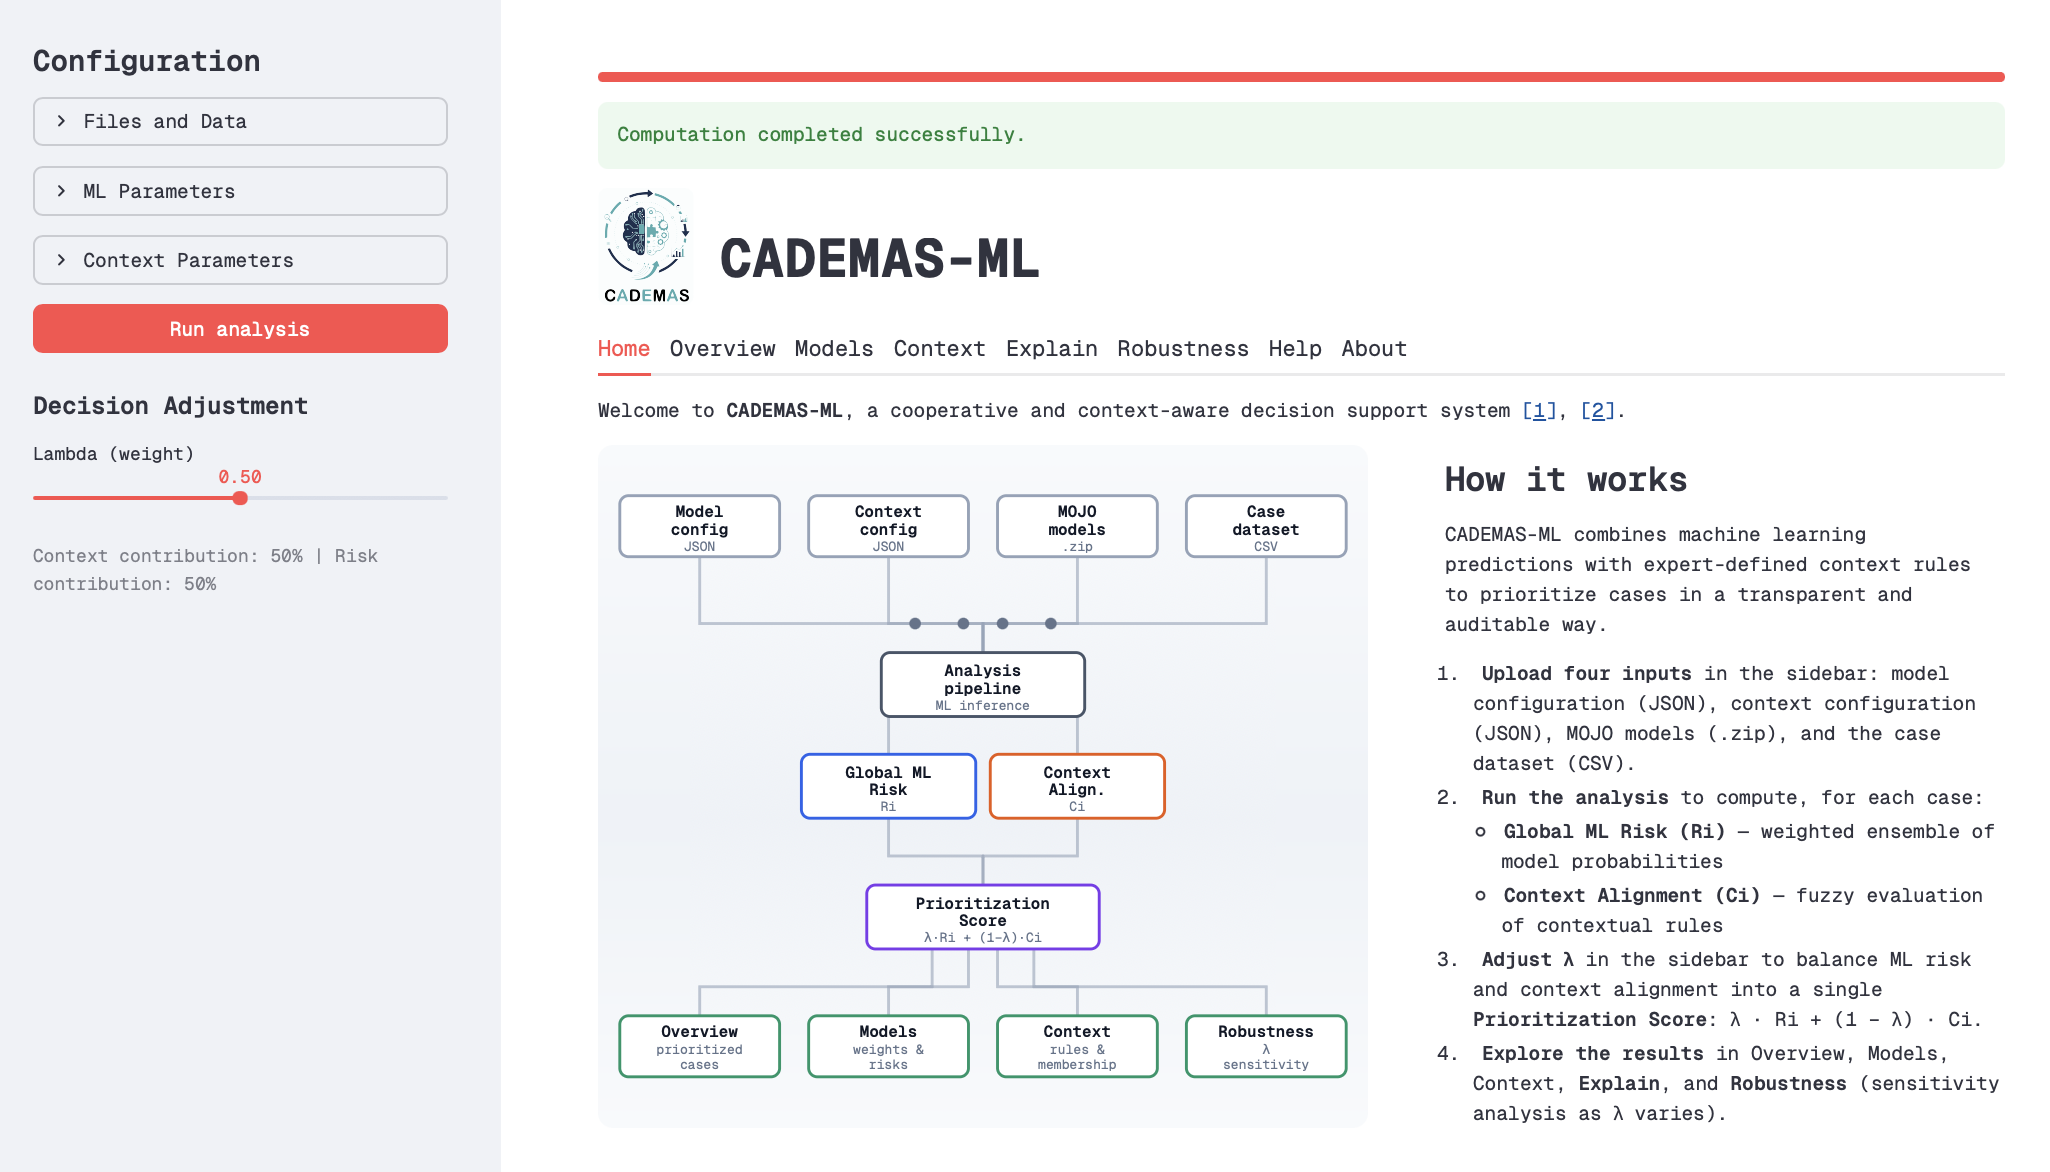
\includegraphics[width=\textwidth,height=0.34\textheight,keepaspectratio]{figures/home.png}
\caption{\textit{Home} and input configuration module. The user uploads or loads the four inputs of Section~\ref{sec:input_manager} and launches the analysis pipeline.}
\label{fig:home_upload}
\end{figure}

\begin{table}[!t]
\tbl{Models used in the attrition example and AUC-based weights computed by CADEMAS-ML. The \textit{AutoML model} column summarizes the artifact exported by H2O AutoML.}
{\footnotesize
\begin{tabularx}{\textwidth}{lllcc}
\toprule
\textbf{ID} & \textbf{Organizational perspective} & \textbf{AutoML model} & \textbf{AUC} & \textbf{Weight} \\
\midrule
$M_1$ & Culture and Wellbeing & Stacked Ensemble (BestOfFamily) & 0.9941 & 0.2623 \\
$M_2$ & Finance & Stacked Ensemble (BestOfFamily) & 0.9972 & 0.2631 \\
$M_3$ & Operations and Development & GBM (grid 1, model 26) & 0.8022 & 0.2116 \\
$M_4$ & Human Resources & Stacked Ensemble (BestOfFamily) & 0.9968 & 0.2630 \\
\bottomrule
\end{tabularx}}
\label{tab:tool_model_weights}
\end{table}

\subsection{\textit{Overview}: integrated prioritization}

After execution, the \textit{Overview} module surfaces the cooperative predictive risk $R_i$ of Equation~\eqref{eq:ml_risk} (Section~\ref{sec:decision_integration}), the context-alignment score $C_i$ of Equation~\eqref{eq:context_score}, and the prioritization score $P_i(\lambda)$ of Equation~\eqref{eq:priority_lambda}. Figure~\ref{fig:overview} shows the exported interface. At the top, the \textit{Prioritization: Risk vs Context} scatter plot locates each case in the $(R_i,C_i)$ plane and encodes $P_i(0.5)$ through color. The adjacent \textit{Prioritization Score} histogram summarizes the cohort-wide distribution of prioritization scores. Below, the \textit{Prioritized Cases} table lists all cases ordered by $P_i(0.5)$, reporting $R_i$, $C_i$, and the \texttt{attrition} outcome label retained for verification only. In this run, $C_i$ ranges from 0.1500 to 0.7100, with a mean of 0.4663. The ten highest-priority cases at $\lambda=0.5$ are used later in the robustness analysis of Figure~\ref{fig:robustness}.

\begin{figure}[!tb]
\centering
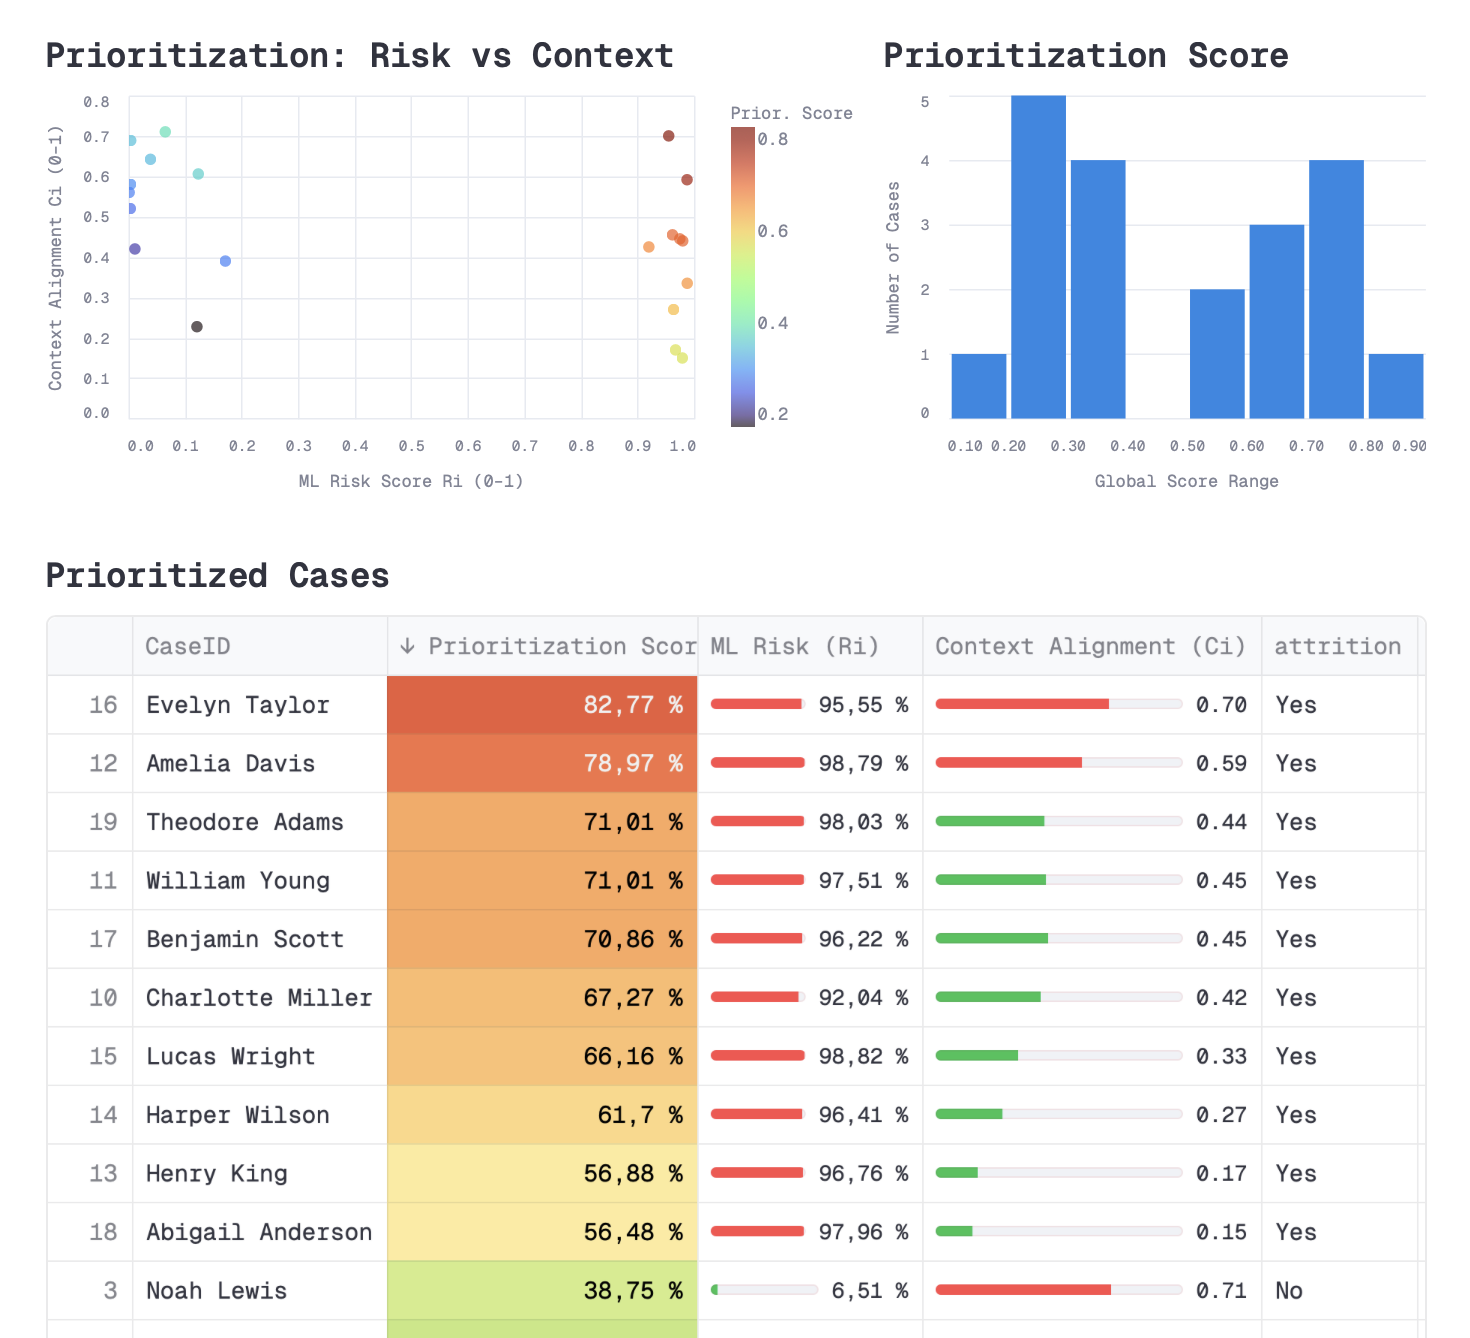
\includegraphics[width=\textwidth]{figures/overview.png}
\caption{\textit{Overview} module for the attrition example at $\lambda=0.5$ in the \textit{Digital / Technological Transformation} context. The scatter plot and histogram summarize the risk--context landscape and the distribution of $P_i(0.5)$; the \textit{Prioritized Cases} table below lists the full cohort by prioritization score, including high-priority employees and context-aligned but low-risk cases such as \textit{Noah Lewis}.}
\label{fig:overview}
\end{figure}

The prioritization ranking in Figure~\ref{fig:overview} is driven primarily by cooperative predictive risk. The highest-priority cases exhibit high $R_i$, while $C_i$ varies more widely. \textit{Evelyn Taylor} leads the ranking because both components are high ($R_i=0.9555$, $C_i=0.7000$), producing $P_i(0.5)=0.8277$. Cases such as \textit{Lucas Wright} and \textit{Abigail Anderson} remain near the top mainly because of critical predictive risk, even though their contextual alignment is moderate or low. By contrast, \textit{Noah Lewis} appears far down the table despite having the highest $C_i$ in the cohort ($C_i=0.7100$). His cooperative predictive risk is low ($R_i=0.0651$), yielding $P_i(0.5)=0.3875$. The juxtaposition of scatter plot, score distribution, and full case table illustrates why CADEMAS-ML reports $P_i(\lambda)$, $R_i$, and $C_i$ separately rather than ranking cases by contextual alignment alone.

\subsection{\textit{Models}: cooperative predictive risk}

The \textit{Models} module exposes the intermediate results of the cooperative predictive-risk layer. Figure~\ref{fig:models} shows the exported interface for the reproduced run. The upper table, \textit{Model Weights}, links each uploaded MOJO to its normalized contribution $w_k$. The values displayed are consistent with those reported in Table~\ref{tab:tool_model_weights}. The lower table, \textit{Risk Probabilities}, reports the per-case positive-class probability returned by each model and the cooperative score $R_i$ in the column immediately after \texttt{CaseID}. Cases are ordered by decreasing $R_i$.

\begin{figure}[!tb]
\centering
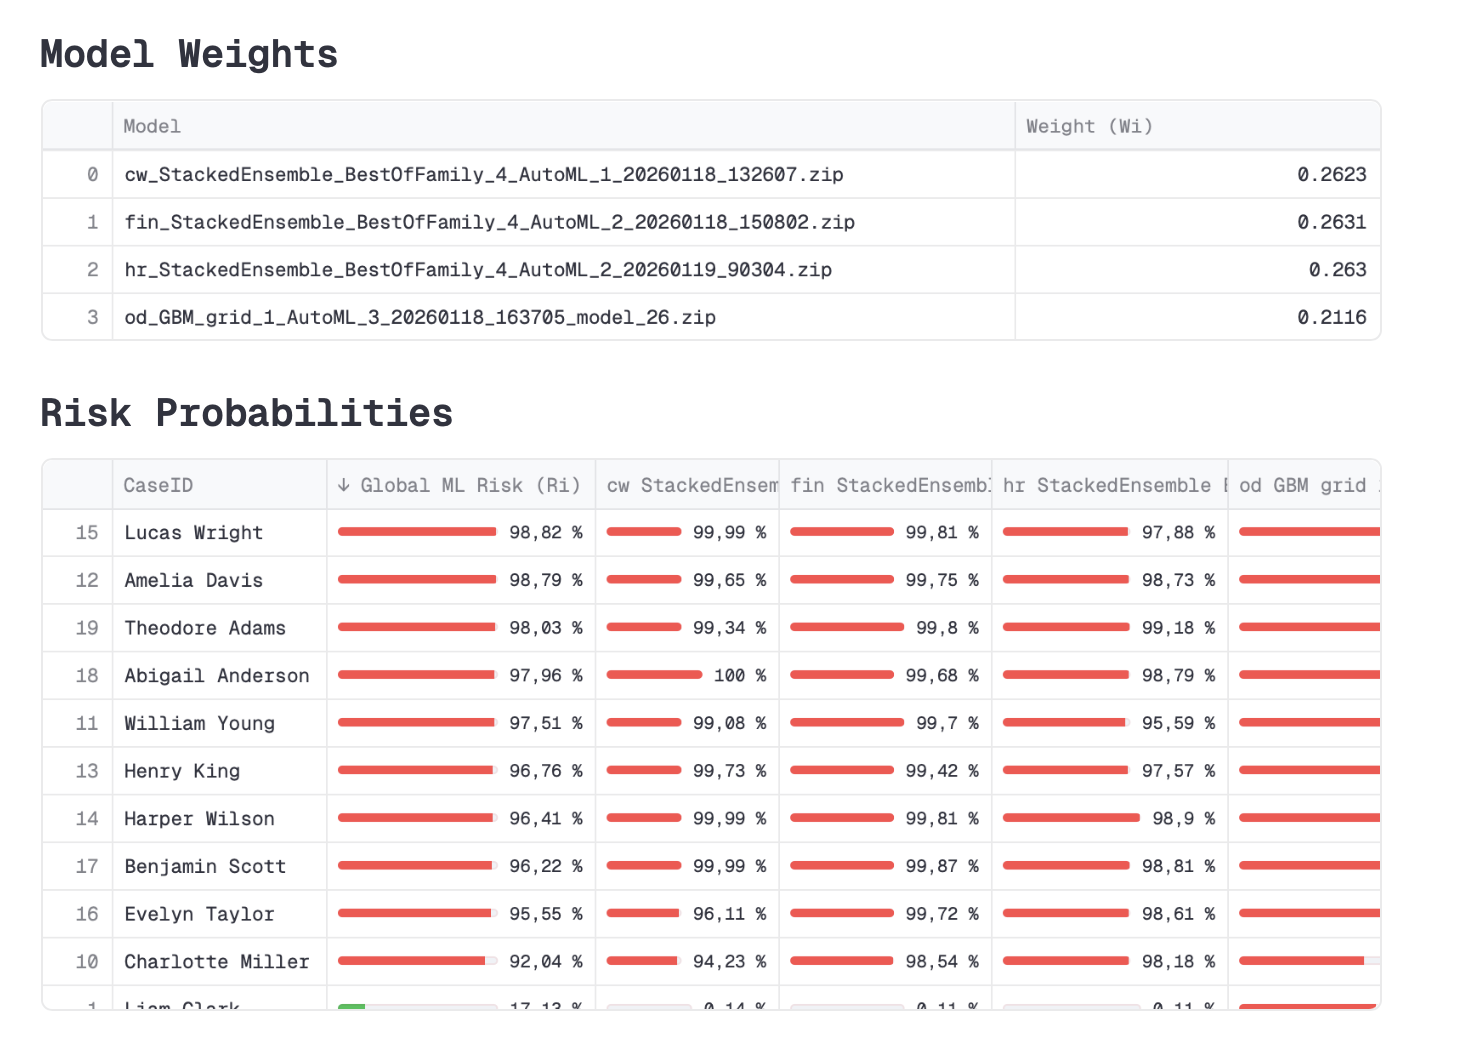
\includegraphics[width=\textwidth]{figures/models.png}
\caption{\textit{Models} module for the attrition example, showing the model-weight table that assigns each MOJO its contribution $w_k$ and, below, the risk-probability table with Global ML Risk ($R_i$), per-model probabilities, and cases sorted by decreasing $R_i$.}
\label{fig:models}
\end{figure}

In the exported view, \textit{Lucas Wright} appears first ($R_i=0.9882$), followed by \textit{Amelia Davis} ($R_i=0.9879$) and \textit{Theodore Adams} ($R_i=0.9803$). This ordering differs from the integrated prioritization in Figure~\ref{fig:overview}, where \textit{Evelyn Taylor} leads because $P_i(0.5)$ also incorporates contextual alignment. The side-by-side per-model columns make the cooperative aggregation auditable. Although all four MOJOs assign high attrition probabilities to the top rows, Operations and Development contributes less to $R_i$ because its validation weight is lower ($w_3=0.2116$). Together, the two tables connect the model-confidence weights $w_k$ to the case-level cooperative predictive risk fed into the prioritization score.

\subsection{\textit{Context}: contextual alignment}

The \textit{Context} module renders the fuzzy audit that produces $C_i$. Figure~\ref{fig:context} exports the interface for the \textit{Digital / Technological Transformation} context. The upper panel lets analysts select an atomic rule and inspect its membership function together with the cohort distribution of the underlying feature, following Equation~\eqref{eq:atomic_mu} (Section~\ref{sec:context_modulator}). A \textit{Numerical Audit} table on the right reports, for each case, the crisp input value and the corresponding membership degree $\mu$. The lower panel, \textit{Derived Rules Overview}, summarizes satisfaction in the composite rules of Equation~\eqref{eq:derived_mu} and the resulting context-alignment score $C_i$ for the full cohort.

\begin{figure}[!tb]
\centering
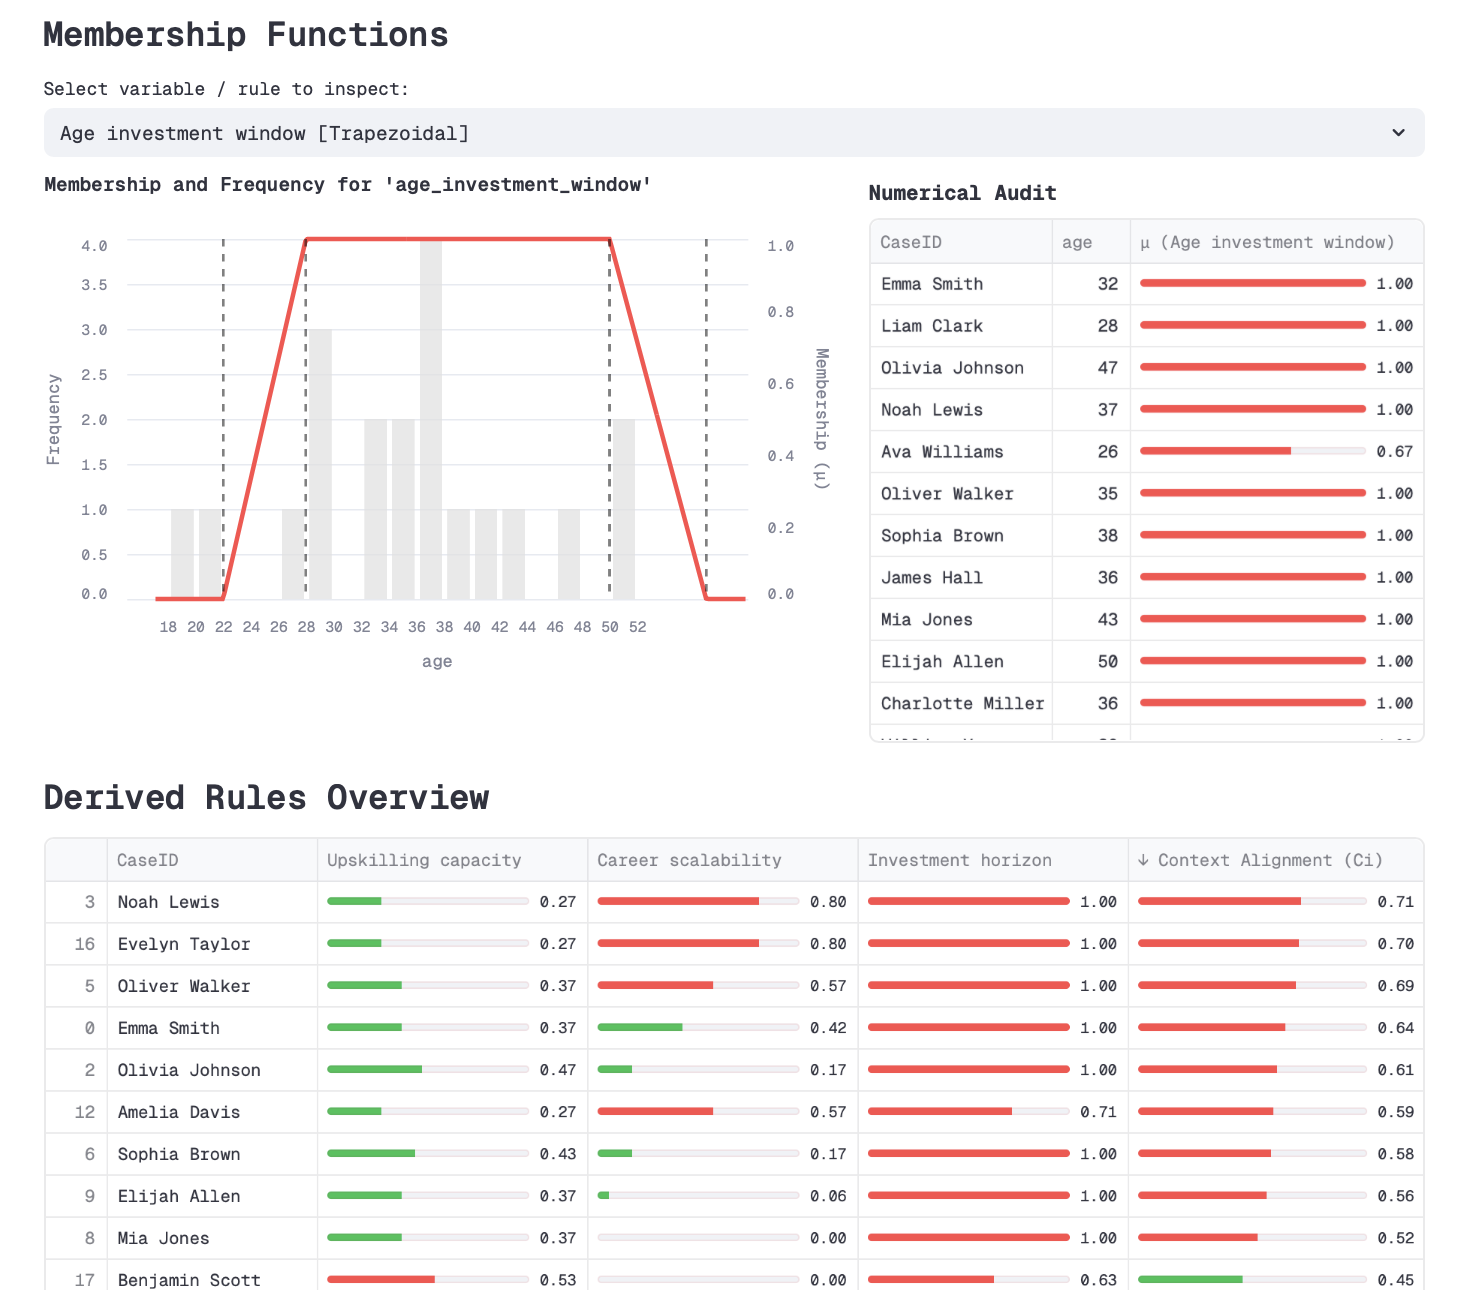
\includegraphics[width=\textwidth]{figures/context.png}
\caption{\textit{Context} module for the \textit{Digital / Technological Transformation} run, combining an atomic-rule selector, the membership-function chart with case distribution, and the numerical audit table for \textit{Age investment window} (trapezoidal), together with a derived-rules overview reporting membership degrees and $C_i$ for cases ordered by decreasing context alignment.}
\label{fig:context}
\end{figure}

In the exported view, the analyst has selected the trapezoidal atomic rule \textit{Age investment window}, which defines the acceptable age range for developmental investment during the transformation program (Appendix~\ref{app:context_specs}). The chart links each employee's age to its membership $\mu$, while the audit table makes the same mapping explicit case by case. Below, \textit{Derived Rules Overview} exposes the degrees of satisfaction for \textit{Upskilling capacity}, \textit{Career scalability}, and \textit{Investment horizon}, together with the aggregated score $C_i$. The table is sorted by $C_i$ in descending order, so \textit{Noah Lewis} ($C_i=0.7100$) appears first and \textit{Evelyn Taylor} ($C_i=0.7000$) second, even though Evelyn leads the integrated ranking in Figure~\ref{fig:overview} because of higher cooperative risk. This view therefore complements the prioritization summary by making the contextual evidence auditable rule by rule and case by case.

\subsection{\textit{Explain}: local case interpretation}

For a selected case, the \textit{Explain} module assembles the four explanation levels defined in Section~\ref{sec:extensions} into a single audit view. Figure~\ref{fig:explain} exports the interface for \textit{Evelyn Taylor}, the highest-priority case in Figure~\ref{fig:overview}. Figure~\ref{fig:explain}-A shows the case selector, the deterministic natural-language summary, and the headline statistics on which that summary rests: $P_i(0.5)$, $R_i$, $C_i$, and $\lambda$, together with the additive decomposition of Equation~\eqref{eq:priority_decomposition}. Figure~\ref{fig:explain}-B reports the aggregated ML attributions of Equations~\eqref{eq:local_attribution_model}--\eqref{eq:local_attribution_global} for the ten most influential features and, below, the fuzzy memberships that trace how strongly each contextual rule is satisfied for the selected case.

\begin{figure}[!tb]
\centering
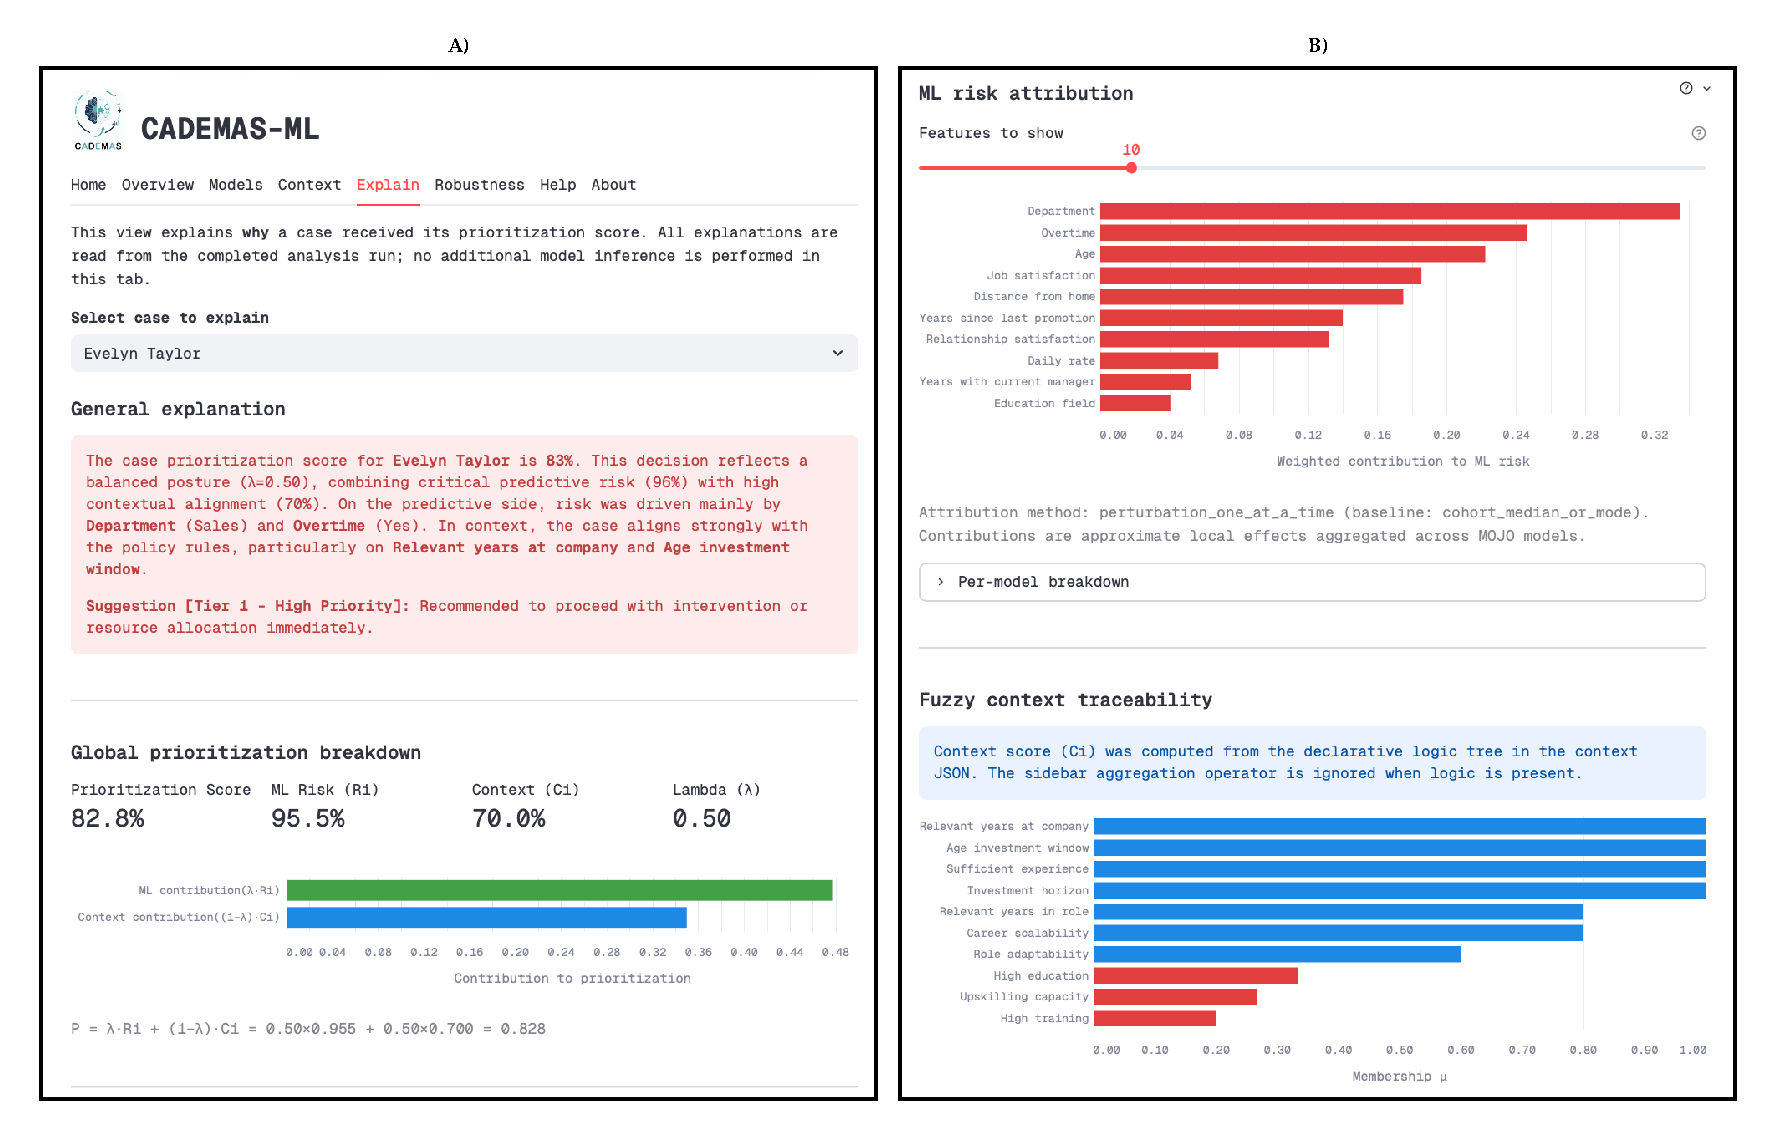
\includegraphics[width=\textwidth]{figures/explain_high_prioritization.pdf}
\caption{\textit{Explain} module for \textit{Evelyn Taylor} at $\lambda=0.5$ in the \textit{Digital / Technological Transformation} context, with case selection, natural-language explanation, summary statistics, aggregated bar charts of the ten most influential ML features, and a fuzzy context traceability panel reporting membership degrees for the policy rules.}
\label{fig:explain}
\end{figure}

Two cases illustrate the interpretation produced by the \textit{Explain} module. The first is \textit{Evelyn Taylor}, ranked first in Figure~\ref{fig:overview} and reproduced in Figure~\ref{fig:explain}. The second is \textit{Noah Lewis}, who ranks low in the same overview despite having the highest $C_i$ in the cohort. For space reasons, only the \textit{Evelyn Taylor} view is shown in the figure. The contrasting \textit{Noah Lewis} summary is reported below in textual form. In both cases, the summaries were reproduced from CADEMAS-ML and follow its deterministic template.

\textit{Evelyn Taylor} combines critical predictive risk ($R_i=0.9555$) with high contextual alignment ($C_i=0.7000$), yielding $P_i(0.5)=0.8277$ and a \textit{Tier 1} recommendation. Figure~\ref{fig:explain}-A displays these values together with the natural-language synthesis. Figure~\ref{fig:explain}-B highlights Department (Sales) and Overtime (Yes) among the strongest ML drivers and shows high membership on Relevant years at company and Age investment window in the fuzzy traceability panel:

\begin{quote}
\small
The case prioritization score for \textit{Evelyn Taylor} is 83\%. This decision reflects a balanced posture ($\lambda=0.50$), combining critical predictive risk (96\%) with high contextual alignment (70\%). On the predictive side, risk was driven mainly by Department (Sales) and Overtime (Yes). In context, the case aligns strongly with the policy rules, particularly on Relevant years at company and Age investment window.

Suggestion [\textit{Tier 1} -- High Priority]: Recommended to proceed with intervention or resource allocation immediately.
\end{quote}

\textit{Noah Lewis} provides a contrasting interpretation. Although this case has the highest contextual alignment in the cohort ($C_i=0.7100$), its cooperative predictive risk is low ($R_i=0.0651$). The resulting prioritization score is therefore $P_i(0.5)=0.3875$, and the module assigns \textit{Tier 3}:

\begin{quote}
\small
The case prioritization score for \textit{Noah Lewis} is 39\%. This decision reflects a balanced posture ($\lambda=0.50$), combining low predictive risk (7\%) with high contextual alignment (71\%). On the predictive side, risk was driven mainly by Years with current manager (8) and Number of companies worked (1). In context, the case aligns strongly with the policy rules, particularly on Relevant years at company and Age investment window.

Suggestion [\textit{Tier 3} -- Low Priority]: Intervention or resource allocation is not justified under current prediction and context guidelines.
\end{quote}

In practical terms, CADEMAS-ML explains not only why a case is prioritized, but also why another case with strong contextual alignment may still receive a low final score when predictive risk remains limited. A third illustrative pattern is provided by \textit{Theodore Adams} ($R_i=0.9803$, $C_i=0.4400$, $P_i(0.5)=0.7101$), who receives \textit{Tier 2} because high predictive risk and only moderate contextual alignment produce borderline evidence under the current policy.

\subsection{\textit{Robustness}: sensitivity of the priority ranking}

The \textit{Robustness} module implements the sensitivity analysis of Section~\ref{sec:extensions}. Figure~\ref{fig:robustness} illustrates the exported Altair charts using $\Lambda=\{0,0.25,0.5,0.75,1\}$ and the ten highest-priority cases at $\lambda=0.5$ (the head of the ranking in Figure~\ref{fig:overview}).

Figure~\ref{fig:robustness}-A shows the bump chart of priority ranks $r_i(\lambda)$ across $\lambda$, following Equation~\eqref{eq:rank_lambda}. Figure~\ref{fig:robustness}-B reports the ranks box plot, which summarizes the rank distribution of each displayed case over the same sweep. Cases are ordered from left to right by median rank and, in case of ties, by interquartile range. Figure~\ref{fig:robustness}-C shows the rank acceptability indices of Equation~\eqref{eq:rank_acceptability}, estimating the relative frequency with which each case occupies each rank position over $\Lambda$.

\begin{figure}[!htb]
  \centering
  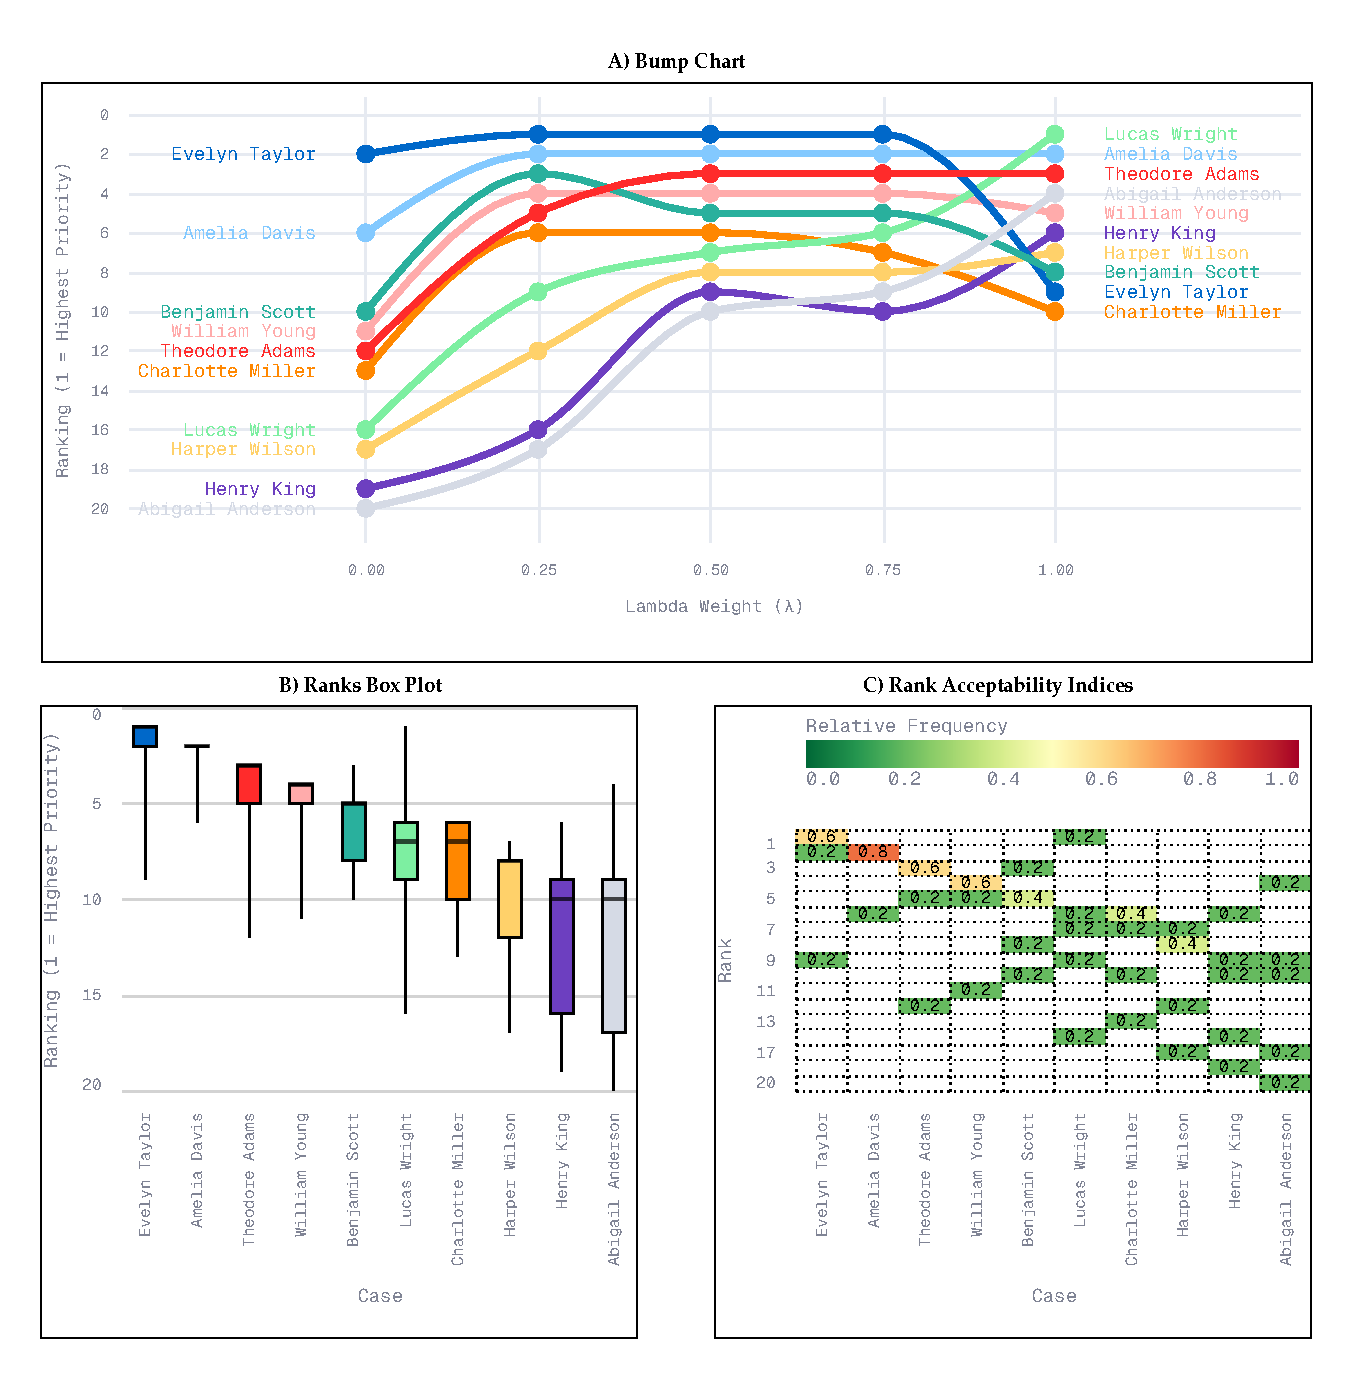
\includegraphics[width=\textwidth]{figures/robustness.pdf}
  \caption{Robustness analysis for the \textit{Digital / Technological Transformation} context exported from CADEMAS-ML over $\Lambda=\{0,0.25,0.5,0.75,1\}$ for the ten highest-priority cases at $\lambda=0.5$, comprising a bump chart of priority ranks across $\lambda$, a ranks box plot of rank distributions over the same sweep, and rank acceptability indices.}
  \label{fig:robustness}
\end{figure}

When $\lambda$ approaches 0 and contextual alignment receives greater weight, cases outside the top ten at $\lambda=0.5$, such as \textit{Noah Lewis} and \textit{Emma Smith}, rise in Figure~\ref{fig:robustness}-A because they combine high $C_i$ with low $R_i$. When $\lambda$ approaches 1, the high-risk cases at the head of Figure~\ref{fig:overview}, such as \textit{Lucas Wright} and \textit{Theodore Adams}, dominate the ranking regardless of transformation alignment. \textit{Evelyn Taylor} remains near the top across intermediate values of $\lambda$ because both $R_i$ and $C_i$ are high. The box plot in Figure~\ref{fig:robustness}-B makes this contrast visible at a glance: stable high-priority cases exhibit compact rank distributions, whereas policy-sensitive cases show wider spreads. Figure~\ref{fig:robustness}-C complements both views by quantifying how often each case attains each rank over the $\lambda$ grid.

\section{Discussion}\label{sec:discussion}

This paper presented CADEMAS-ML as an executable specialization of the CADEMAS framework for cooperative, context-aware, ML-based prioritization. Its contribution is not a new attrition predictor, but an operational separation of predictive evidence, contextual evaluation, and final prioritization. This separation builds on the general architecture of \citet{NovoaHernandez2026} and the employee-attrition instantiation of \citet{Godz2026}, while adding reusable configuration, case-level explanation, and ranking-sensitivity analysis. The employee-attrition case study shows the practical consequence of that design: rankings based on cooperative predictive risk need not coincide with rankings based on contextual alignment, and the explicit combination of both can be inspected rather than treated as an opaque post-processing step.

The tool also occupies a distinct position relative to related decision-support software. Existing platforms and libraries have made important advances in exposing intermediate fuzzy or multi-criteria calculations \citep{Wieckowski2024,Chekry2024}, while hybrid approaches have combined prediction, ranking, expert knowledge, and explainability in application-specific pipelines \citep{Ozkurt2025}. CADEMAS-ML complements these contributions by organizing the workflow around cooperating ADM units and by keeping their integrated output separate from the context in which a decision is made. The \textit{Models}, \textit{Context}, and \textit{Overview} views preserve this distinction; the \textit{Explain} and \textit{Robustness} views then support case-level interpretation and policy-sensitivity analysis. These additions extend the static prioritization workflow considered in earlier CADEMAS work.

For practitioners, the main benefit of this architecture is the ability to revise decision policy without embedding that policy in the predictive models themselves. When organizational conditions change, analysts can retain the predictive layer, provide a different context specification, and examine how the resulting priorities change. The separate reporting of $R_i$, $C_i$, and $P_i(\lambda)$ makes the source of a recommendation visible, while the $\lambda$ sweep identifies cases whose position is stable and cases whose priority depends strongly on the selected balance. This does not remove the need for professional judgment; rather, it provides a structured record of the predictive and policy assumptions presented to the decision-maker. Potential applications include alert triage, review queues, retention programs, and allocation of limited support or inspection resources, provided that models, contextual rules, and decision thresholds are validated for the domain concerned.

For researchers, CADEMAS-ML provides a reproducible environment in which alternative cooperation, context-representation, explanation, and robustness mechanisms can be compared within a common architecture. The current implementation uses performance-normalized weights to combine independently trained models and a convex linear rule, $P_i(\lambda)=\lambda R_i+(1-\lambda)C_i$, to integrate predictive risk and context. This final rule is compensatory: sufficiently strong evidence in one component can offset weaker evidence in the other. Recent work on aggregation semantics for CADEMAS \citep{novoa2026aggregation} motivates extending the software with operator families that express different compensation requirements, including conjunctive or veto-like behavior. Making the aggregation semantics configurable would allow the software to distinguish settings in which compensation is acceptable from those in which a minimum level of predictive or contextual support is required.

A related direction is to move cooperation upstream, from post-hoc output aggregation to model development. At present, the predictive ADM units are trained independently and cooperation begins when their probabilities are weighted. Future versions could investigate diversity-aware model selection, theory-informed learning constraints, or multi-objective procedures that balance predictive performance, calibration, and complementarity. The aim would not be to encourage disagreement for its own sake, but to obtain models that remain individually reliable while contributing non-redundant evidence from different variables, data sources, or perspectives on the problem. Measures of conditional competence and redundancy could then inform both training and aggregation, providing a more principled trade-off between the performance of individual ADM units and the informational value of their cooperation.

Several limitations delimit these implications. The ADM units currently supported at run time are H2O MOJO classifiers; the broader CADEMAS notion of heterogeneous units, including optimization models, simulators, or rule-based systems, is not yet implemented. Local ML attributions are model-agnostic perturbations around a cohort baseline and should not be read as causal effects or as substitutes for model-specific explanation methods when model internals are available. The attrition case study uses a 20-case illustrative subset and is neither a predictive-performance study nor evidence for general human-resources policy. Moreover, context specifications require domain-expert elicitation, and the interface does not yet provide versioned approval workflows or immutable audit trails for production governance. Future development should therefore combine broader ADM support and richer aggregation semantics with empirical validation in additional domains, stronger context governance, and evaluation with the practitioners who would interpret and act on the resulting priorities.

\section*{Funding}

This research was supported by the project ``Study, Analysis and Evaluation of Cooperative Automated Decision-Making Systems (CADEMAS)'', PID2023-146575NB-I00, funded by MCIU/AEI/10.13039/501100011033 and by FEDER, EU.

\section*{Disclosure statement}

The authors report there are no competing interests to declare.

\section*{Declaration of generative AI use}

Generative AI tools were used to assist with language editing and manuscript formatting. The authors reviewed and take full responsibility for the content of this article.

\section*{Data availability statement}

The illustrative employee records used in this article are a 20-case subset derived from the publicly available IBM HR Analytics Employee Attrition and Performance dataset \citep{IBMHRKaggle}. The subset, model metadata, MOJO archives, and context specifications are distributed with the software repository cited in Section~\ref{sec:software}.

\phantomsection
\section*{Software availability}\label{sec:software}

CADEMAS-ML is available at \url{https://github.com/pnovoa/cademas-app} under an MIT license \citep{cademasml2026}. An archival snapshot will be deposited in Zenodo at the time of submission; the corresponding DOI will be inserted when it is available.

\section*{Supplementary material}

Supplementary Material~S1 accompanies this article and provides the complete specification of the four application inputs, field-level constraints, cross-file consistency requirements, and minimal configuration examples.

\section*{Author contributions}  

Pavel Novoa-Hern\'{a}ndez: conceptualization, methodology, software, validation, writing -- original draft, visualization. David A. Pelta: conceptualization, methodology, supervision, writing -- review and editing.

\bibliographystyle{apacite}
\bibliography{biblio}

\section*{Notes on contributors}

\noindent\textbf{Pavel Novoa-Hern\'{a}ndez} is Associate Professor in the Department of Computer Engineering and Systems at Universidad de La Laguna, Spain. His research interests include automated decision-making, decision-making under uncertainty, evolutionary computation, and machine learning applications.

\noindent\textbf{David A. Pelta} is Full Professor in the Department of Computer Science and Artificial Intelligence at Universidad de Granada, Spain. His research focuses on fuzzy optimization, evolutionary computation, and decision-making under uncertainty.

\appendix
\section{Attrition example dataset and model features}\label{app:attrition_features}

The 20-case attrition example distributed with CADEMAS-ML contains 36 columns: \texttt{Case\_ID}, 34 predictor variables, and the \texttt{attrition} outcome label. The predictors cover demographic, professional, compensation, performance, and organizational attributes from the \textit{IBM HR Analytics Employee Attrition and Performance} Kaggle dataset used in \citet{Godz2026}. Five variables (\texttt{age}, \texttt{gender}, \texttt{department}, \texttt{job\_role}, and \texttt{job\_level}) are shared by all four MOJO models. Two additional columns (\texttt{employee\_count} and \texttt{employee\_number}) are retained in the CSV file but are not used by any model in the example bundle. Each MOJO receives the full case matrix and selects its required variables according to the schema stored in the model-definition JSON file.

Table~\ref{tab:attrition_feature_assignment} summarizes the feature assignment. The Human Resources model reads \texttt{over18} from the CSV file; the corresponding field is named \texttt{over\_18} in the model metadata.

\begin{table}[!tbh]
\tbl{Predictor variables in the attrition example and the MOJO models that use each one. $M_1$--$M_4$ denote Culture and Wellbeing, Finance, Operations and Development, and Human Resources, respectively.}
{\footnotesize
\begin{tabularx}{\textwidth}{%
  >{\raggedright\arraybackslash\ttfamily}X
  >{\centering\arraybackslash}p{1.55cm}
  >{\centering\arraybackslash}p{1.55cm} 
  >{\centering\arraybackslash}p{1.55cm}
  >{\centering\arraybackslash}p{1.55cm}
}
\toprule
\multicolumn{1}{l}{\normalfont\textbf{Predictor}} &
\textbf{\boldmath$M_1$} &
\textbf{\boldmath$M_2$} &
\textbf{\boldmath$M_3$} &
\textbf{\boldmath$M_4$} \\
& {\scriptsize Culture \& Wellbeing} &
{\scriptsize Finance} &
{\scriptsize Ops.\ \& Dev.} &
{\scriptsize Human Resources} \\
\midrule
age & $\checkmark$ & $\checkmark$ & $\checkmark$ & $\checkmark$ \\
business\_travel & $\checkmark$ &  &  &  \\
daily\_rate &  & $\checkmark$ &  &  \\
department & $\checkmark$ & $\checkmark$ & $\checkmark$ & $\checkmark$ \\
distance\_from\_home &  &  &  & $\checkmark$ \\
education &  &  &  & $\checkmark$ \\
education\_field &  &  &  & $\checkmark$ \\
employee\_count &  &  &  &  \\
employee\_number &  &  &  &  \\
environment\_satisfaction & $\checkmark$ &  &  &  \\
gender & $\checkmark$ & $\checkmark$ & $\checkmark$ & $\checkmark$ \\
hourly\_rate &  & $\checkmark$ &  &  \\
job\_involvement & $\checkmark$ &  &  &  \\
job\_level & $\checkmark$ & $\checkmark$ & $\checkmark$ & $\checkmark$ \\
job\_role & $\checkmark$ & $\checkmark$ & $\checkmark$ & $\checkmark$ \\
job\_satisfaction & $\checkmark$ &  &  &  \\
marital\_status &  &  &  & $\checkmark$ \\
monthly\_income &  & $\checkmark$ &  &  \\
monthly\_rate &  & $\checkmark$ &  &  \\
num\_companies\_worked &  &  & $\checkmark$ &  \\
over18 &  &  &  & $\checkmark$ \\
over\_time & $\checkmark$ &  &  &  \\
percent\_salary\_hike &  & $\checkmark$ &  &  \\
performance\_rating &  &  & $\checkmark$ &  \\
relationship\_satisfaction & $\checkmark$ &  &  &  \\
standard\_hours &  &  &  & $\checkmark$ \\
stock\_option\_level &  & $\checkmark$ &  &  \\
total\_working\_years &  &  & $\checkmark$ &  \\
training\_times\_last\_year &  &  & $\checkmark$ &  \\
work\_life\_balance & $\checkmark$ &  &  &  \\
years\_at\_company &  &  & $\checkmark$ &  \\
years\_in\_current\_role &  &  & $\checkmark$ &  \\
years\_since\_last\_promotion &  &  & $\checkmark$ &  \\
years\_with\_curr\_manager &  &  & $\checkmark$ &  \\
\midrule
\multicolumn{1}{l}{\normalfont\textbf{Total features}} & 12 & 11 & 13 & 11 \\
\bottomrule
\end{tabularx}}
\label{tab:attrition_feature_assignment}
\end{table}

\section{Context specification for the \textit{Digital / Technological Transformation} scenario}\label{app:context_specs}

The example repository includes two context configurations, but the walkthrough focuses on \textit{Digital / Technological Transformation}. This appendix reports the corresponding fuzzy specification in closed form so that every membership degree and the final context-alignment score $C_i$ can be audited without inspecting application code. The rules instantiate the generic formalism of Equations~\eqref{eq:atomic_mu}--\eqref{eq:context_score}; equivalent parameters are stored in the repository JSON file consumed by CADEMAS-ML\footnote{\url{https://github.com/pnovoa/cademas-app/blob/main/example_attrition/context/context_digital_transformation.json}.}. They are illustrative policy encodings, not hard-coded assumptions of the tool.

\subsection{Generic membership functions}\label{app:context_math_mf}

Each numerical atomic rule is evaluated through one of four parametric membership functions. For an input value $x$, the \emph{linear increasing} function with breakpoints $(a,b)$, $a<b$, is
\begin{equation}
\mu^{\uparrow}_{a,b}(x)=
\begin{cases}
0, & x \le a,\\[2pt]
\dfrac{x-a}{b-a}, & a < x < b,\\[6pt]
1, & x \ge b,
\end{cases}
\label{eq:mf_linc}
\end{equation}
and the \emph{linear decreasing} function with breakpoints $(a,b)$ is its mirror image
\begin{equation}
\mu^{\downarrow}_{a,b}(x)=1-\mu^{\uparrow}_{a,b}(x)=
\begin{cases}
1, & x \le a,\\[2pt]
\dfrac{b-x}{b-a}, & a < x < b,\\[6pt]
0, & x \ge b.
\end{cases}
\label{eq:mf_ldec}
\end{equation}
The \emph{triangular} function with support $(a,c)$ and peak $b$, $a<b<c$, is
\begin{equation}
\operatorname{tri}_{a,b,c}(x)=
\begin{cases}
\dfrac{x-a}{b-a}, & a < x \le b,\\[6pt]
\dfrac{c-x}{c-b}, & b < x < c,\\[6pt]
0, & \text{otherwise},
\end{cases}
\label{eq:mf_tri}
\end{equation}
and the \emph{trapezoidal} function with feet $(a,d)$ and shoulders $(b,c)$, $a<b\le c<d$, is
\begin{equation}
\Pi_{a,b,c,d}(x)=
\begin{cases}
\dfrac{x-a}{b-a}, & a < x < b,\\[6pt]
1, & b \le x \le c,\\[2pt]
\dfrac{d-x}{d-c}, & c < x < d,\\[6pt]
0, & \text{otherwise}.
\end{cases}
\label{eq:mf_trap}
\end{equation}
Categorical attributes are handled by a direct map $\kappa:\mathcal{S}\to[0,1]$ that assigns a degree to each symbolic value $s\in\mathcal{S}$, with unspecified categories defaulting to $0$.

\subsection{Atomic rules}\label{app:context_math_atomic}

Seven atomic rules evaluate recent training intensity, education level, company tenure, tenure in the current role, age in the investment window, accumulated experience, and role adaptability to technological change. For case $x_i$, the corresponding memberships are
\begin{align}
\mu_{\textsf{train}}(x_i) &= \mu^{\uparrow}_{1,6}\!\left(\textsf{training\_times\_last\_year}_i\right), \label{eq:atom_train}\\
\mu_{\textsf{edu}}(x_i) &= \mu^{\uparrow}_{2,5}\!\left(\textsf{education}_i\right), \label{eq:atom_edu}\\
\mu_{\textsf{yrsCo}}(x_i) &= \operatorname{tri}_{3,10,20}\!\left(\textsf{years\_at\_company}_i\right), \label{eq:atom_yrsco}\\
\mu_{\textsf{yrsRole}}(x_i) &= \operatorname{tri}_{1,6,11}\!\left(\textsf{years\_in\_current\_role}_i\right), \label{eq:atom_yrsrole}\\
\mu_{\textsf{age}}(x_i) &= \Pi_{22,28,50,57}\!\left(\textsf{age}_i\right), \label{eq:atom_age}\\
\mu_{\textsf{exp}}(x_i) &= \mu^{\uparrow}_{2,10}\!\left(\textsf{total\_working\_years}_i\right), \label{eq:atom_exp}\\
\mu_{\textsf{role}}(x_i) &= \kappa_{\textsf{role}}\!\left(\textsf{job\_role}_i\right), \label{eq:atom_role}
\end{align}
where the role-adaptability map assigns expert scores to each job role:
\begin{equation}
\kappa_{\textsf{role}}(s)=
\begin{cases}
0.9, & s\in\{\text{Research Scientist},\ \text{Research Director}\},\\
0.8, & s=\text{Manager},\\
0.7, & s\in\{\text{Manufacturing Director},\ \text{Healthcare Representative}\},\\
0.6, & s=\text{Sales Executive},\\
0.5, & s=\text{Human Resources},\\
0.4, & s\in\{\text{Laboratory Technician},\ \text{Sales Representative}\}.
\end{cases}
\label{eq:kappa_role}
\end{equation}
Each expression can be read directly: for instance, Equation~\eqref{eq:atom_age} states that ages between 28 and 50 fully satisfy the investment window ($\mu=1$), the degree decays linearly toward the feet at 22 and 57, and ages outside $[22,57]$ are excluded.

\subsection{Derived rules and final aggregation}\label{app:context_math_derived}

The aggregation operators of Equation~\eqref{eq:derived_mu}, applied to a vector $\mathbf{u}=(u_1,\ldots,u_q)$, are
\begin{equation}
\textsc{and}(\mathbf{u})=\min_{j} u_j,\quad
\textsc{or}(\mathbf{u})=\max_{j} u_j,\quad
\textsc{prod}(\mathbf{u})=\prod_{j=1}^{q} u_j,\quad
\textsc{avg}(\mathbf{u})=\frac{1}{q}\sum_{j=1}^{q} u_j.
\label{eq:agg_ops}
\end{equation}
With these operators, three derived criteria combine the atomic memberships: \emph{upskilling capacity} (training and education), \emph{career scalability} (company and role tenure), and \emph{investment horizon} (age window and experience). Formally,
\begin{align}
\mu_{\textsf{upskill}}(x_i) &= \textsc{avg}\!\left(\mu_{\textsf{train}}(x_i),\,\mu_{\textsf{edu}}(x_i)\right)
= \tfrac{1}{2}\!\left(\mu_{\textsf{train}}(x_i)+\mu_{\textsf{edu}}(x_i)\right), \label{eq:der_upskill}\\
\mu_{\textsf{career}}(x_i) &= \textsc{prod}\!\left(\mu_{\textsf{yrsCo}}(x_i),\,\mu_{\textsf{yrsRole}}(x_i)\right)
= \mu_{\textsf{yrsCo}}(x_i)\,\mu_{\textsf{yrsRole}}(x_i), \label{eq:der_career}\\
\mu_{\textsf{invest}}(x_i) &= \textsc{prod}\!\left(\mu_{\textsf{age}}(x_i),\,\mu_{\textsf{exp}}(x_i)\right)
= \mu_{\textsf{age}}(x_i)\,\mu_{\textsf{exp}}(x_i). \label{eq:der_invest}
\end{align}
The choice of operator carries a clear semantics: \textsc{avg} lets strong training compensate for weaker formal education in \emph{upskilling capacity}, whereas the \textsc{prod} operator in \emph{career scalability} and \emph{investment horizon} is conjunctive, so a near-zero membership in either input collapses the derived degree toward zero. The context JSON also identifies four high-level criteria---upskilling, role adaptability, career scalability, and investment horizon---that can be evaluated as a declarative logic tree when no aggregation override is supplied.

In the reported demonstration, the \textit{average} operator is selected explicitly in the user interface. This setting takes precedence over the declarative logic tree and averages all numeric atomic and derived memberships retained in the audit matrix. Let
\[
\mathcal{S}=\{\textsf{train},\textsf{edu},\textsf{yrsCo},\textsf{yrsRole},
\textsf{age},\textsf{exp},\textsf{role},\textsf{upskill},\textsf{career},\textsf{invest}\}.
\]
The context-alignment score used in the figures and numerical results is therefore
\begin{equation}
C_i=\frac{1}{|\mathcal{S}|}\sum_{r\in\mathcal{S}}\mu_r(x_i)
=\frac{1}{10}\sum_{r\in\mathcal{S}}\mu_r(x_i).
\label{eq:context_score_digital}
\end{equation}
Equation~\eqref{eq:context_score_digital} is the explicit instance of the generic policy in Equation~\eqref{eq:context_score} used for this run and defines the contextual evidence surfaced in the \textit{Context} module (Figure~\ref{fig:context}) and traced at case level in the \textit{Explain} module. Selecting \textit{minimum (strict)} or \textit{product} in the interface applies the corresponding operator to the same audit-matrix columns.

\section{Input files and consistency requirements}\label{app:input_summary}

CADEMAS-ML requires four coordinated inputs. Table~\ref{tab:input_contract} summarizes their roles and principal constraints; Supplementary Material~S1 gives the complete field-level specification and minimal examples. The specification distinguishes fields required for scoring from metadata used for display and explanation.

\begin{table}[!tbh]
\tbl{Summary of the CADEMAS-ML input contract.}
{\begin{tabularx}{\textwidth}{>{\raggedright\arraybackslash}p{2.6cm} >{\raggedright\arraybackslash}X >{\raggedright\arraybackslash}X}
\toprule
\textbf{Input} & \textbf{Required content} & \textbf{Cross-file constraints} \\
\midrule
Case dataset (CSV) &
One row per case and columns required by the uploaded models and context rules. A \texttt{Case\_ID} or \texttt{ID} column is optional; otherwise, identifiers are generated. &
Column names and data types must be compatible with the MOJO schemas. Every feature referenced by a context rule must be present. Identifier columns are excluded from inference. \\
\addlinespace
Model metadata (JSON) &
One top-level object per model, containing a \texttt{performance} object. The bundled schema also records \texttt{department} and \texttt{features}; the latter is needed for the perturbation-based explanation workflow. &
Each top-level key must exactly match an uploaded MOJO filename. The metric selected for weighting must be available for every participating model and should be a finite non-negative value. \\
\addlinespace
Predictive models &
H2O MOJO archives in \texttt{.zip} format that return compatible positive-class probabilities. &
Each archive must have a matching metadata entry. All models must use the same positive-class interpretation, although their predictor subsets may differ. \\
\addlinespace
Context specification (JSON) &
A context name, atomic \texttt{rules}, optional \texttt{derived\_rules}, and an optional final \texttt{logic} tree. Rules identify a feature, membership type, parameters, and optionally an activation condition. &
Rule names must be unique, references in derived or final rules must resolve, and parameter shapes must match the membership type. The aggregation operator selected in the interface overrides the final JSON logic for that run. \\
\bottomrule
\end{tabularx}}
\label{tab:input_contract}
\end{table}

The application checks filename matching and loads the selected metric at run time, but publication-quality deployments should validate the complete bundle before analysis. Such validation includes checking finite metric values, membership-parameter ordering, unresolved rule references, missing features, incompatible categorical values, and agreement on the positive class. Keeping these constraints explicit is important because the four files jointly define the executable decision model: none of them is fully interpretable in isolation.

\end{document}
